\chapter{Systematic Uncertainties and Results}

\label{ch:results}
% --------------------------------------------------------------------------------

\section{Systematic Uncertainties}

A number of systematic uncertainties affect the interpretation of the results of the search.
These uncertainties can broken down into two major categories, those which affect the estimate of the background using data and those which affect the measurement of the signal yield estimated with simulated events.
The total measured systematic uncertainties are 7\% for the background estimation and approximately 32\% for the signal yield depending on lifetime.
These systematic uncertainties are expected to be small compared to the statistical fluctuations of the measured yields so that measured cross-sectional limits will be dominated by statistical uncertainties.
The following sections describe each source of systematic uncertainty for each of the two types.

\subsection{Background Estimate}

The systematic uncertainties on the background estimate come primarily from considering alternative methods for generating the background distributions.
These uncertainties are small compared to the statistical uncertainties on the background estimate which come from the limited statistics in measuring the template distributions, as described in Section~\ref{sec:background_method}.
They are summarized in Table~\ref{tab:background_systematics}.

\begin{table}[!htbp]
\begin{center}
  \begin{tabular}{lr}
    \hline
    Source of Uncertainty: &  Value [\%]\\
    \hline
    Analytic Description of \dedx      & 4.0\\	
    Muon Fraction (Stable Region only) & 3.0\\	     
    IBL Ionization Correction          & 3.8 \\	
    Normalization                      & 3.0 \\
    \hline
    Total (Metastable Region): & 6.3\\
    Total (Stable Region):     & 7.0\\
    \hline
  \end{tabular}
\end{center}
\caption{A summary of the sources of systematic uncertainty for the data-driven background in the signal region. If the uncertainty depends on the mass,  the  maximum values are  reported. }
\label{tab:background_systematics}
\end{table}

\subsubsection{Analytic Description of \dedx}

The background estimate uses a binned template distribution to estimate the \dedx of tracks in the signal region, as described in Section~\ref{sec:background_method}.
It is also possible to fit that measured distribution to a functional form to help smooth the distribution in the tails of \dedx where the template is driven by a small number of tracks.
Both Landau convolved with a Gaussian and Crystal Ball functions are considered as the functional form and used to re-estimate the background distribution.
The deviations compared to the nominal method are found to be 4\%, and this is taken as a systematic uncertainty to cover the inability carefully predict the contribution from the long tail of \dedx where there are few measurements available in data.

\subsubsection{Muon Fraction}

The stable region of the analysis explicitly includes tracks identified as muons, which have a known difference in their \dedx distributions compared to non-muon tracks (Section~\ref{sec:background_sources}).
To account for a difference in muon fraction between the background region and the signal region for this selection, the \dedx templates for muons and non-muons are measured separately and then the relative fraction of each is varied in the random generation.
The muon fraction is varied by its statistical uncertainty and the resulting difference of 3\% in background yield is taken as the systematic uncertainty.

\subsubsection{\acs{IBL} Corrections}

The \ac{IBL}, described in Section~\ref{sec:pixel}, received a significant dose of radiation during the data collection in 2015.
The irradiation can cause a drift in the frontend electronics and thus alter the \dedx measurement which includes the \ac{ToT} output by the \ac{IBL}.
These effects are corrected for in the nominal analysis by scaling the \dedx measurements by a constant factor derived for each run to match the average \dedx value to a reference run where the \ac{IBL} was known to be stable to this effect.
However, this corrective factor does not account for inter-run variations.
To account for this potential drift of \dedx, the correction procedure is repeated by varying the corrections up and down by the maximal run-to-run variation from the full data-taking period, which results in an uncertainty of 3.8\%.

\subsubsection{Normalization}

As described in Section~\ref{sec:background_method}, the generated distribution of masses is normalized in a shoulder region ($M < 160$ \GeV) where signals have been excluded by previous analyses.
That normalization factor is varied by its statistical uncertainty and the resulting fluctuation in the mass distribution of 3\% is taken as a systematic uncertainty on the background estimate.

\subsection{Signal Yield}

The systematic uncertainties on the signal yield can be divided into three categories; those on the simulation process, those on the modeling of the detector efficiency or calibration, and those affecting the overall signal yield.
They are summarized in Table~\ref{tab:background_systematics}.
The largest uncertainty comes from the uncertainty on the production cross section for gluinos, which is the dominant systematic uncertainty in this analysis.

\begin{table}[!htbp]
\begin{center}
  \begin{tabular}{lcc}
    \hline
    Source of Uncertainty & $-$[\%]& $+$[\%]\\
    \hline
    ISR Modeling (Metastable Region) & 1.5 & 1.5 \\
    ISR Modeling (Stable Region)     & 14  & 14  \\
    Pile-up Reweighting              & 1.1 & 1.1 \\
    \hline
    Trigger Efficiency Reweighting   & 0.9 & 0.9 \\
    \met Scale                       & 1.1 & 2.2 \\
    Ionization Parametrization      & 7.1 & 0   \\
    Momentum Parametrization        & 0.3 & 0.0 \\
    Electron Rejection               & 0.0 & 0.0 \\
    Hadron Rejection                 & 0.0 & 0.0 \\
    $\mu$~Identification             & 4.3 & 4.3 \\
    \hline   
    Luminosity                       & 5   & 5   \\
    Signal size uncertainty          & 28  & 28  \\
    \hline
    Total (Metastable Region)        & 30  & 29  \\
    Total (Stable Region)            & 33  & 32  \\
    \hline
  \end{tabular}
\end{center}
\caption{A summary of the sources of systematic uncertainty for the simulated signal yield. The uncertainty depends on the mass and lifetime, and the maximum negative and positive values are reported in the table.}
\label{tab:yield_systematics}
\end{table}

\subsubsection{\ac{ISR} Modeling}
As discussed in Section~\ref{sec:simulation_samples}, \texttt{MadGraph} is expected to reproduce the distribution of \ac{ISR} in signal events more accurately than the nominal \texttt{Pythia} samples.
The analysis reweights the distribution of \ac{ISR} in the simulated signal events to match the distribution found in generated \texttt{MadGraph} samples.
This has an effect on the selection efficiency in the signal samples, where \ac{ISR} contributes to the generation of \met.
To account for the potential inaccuracy on the simulation of \ac{ISR} at high energies, half of the difference between the signal efficiency with the reweighted distribution and the original distribution is taken as a systematic uncertainty.

\subsubsection{Pileup Reweighting}
The simulated events were generated prior to data collection with an estimate of the average number of interactions per bunch crossing.
This estimate does not match the value of pileup during actual data collection, but a large fraction of the simulated events would be discarded in order to match the distribution in data.
Therefore the simulated signal events are not reweighted for pileup by default in the analysis.
The effect of the pileup on signal efficiency is not expected to depend on the mass or lifetime of the generated signal events, which allows all of the generated signal events to be used together to assess the pileup dependence.
To account for the potential effect of the difference in the number of interactions per bunch crossing between data and simulation, the difference in yield between the nominal signal events and the reweighted events averaged over all masses and lifetimes is taken as a systematic uncertainty on the yield for each mass and lifetime (1.1\%).

\subsubsection{Trigger Efficiency Reweighting}
As described in Section~\ref{sec:track_requirements}, the selection for this analysis does not require a sufficiently large value of \met to be above the plateau of trigger efficiency.
Therefore, some signal events which would otherwise pass the event selection can be excluded because of the trigger requirement.
These effects can be difficult to estimate in simulation, and thus are constrained by comparing data and simulated events in an alternative W boson region which uses decays to muons to find a relatively pure sample of events with missing energy.
The trigger efficiency for data and simulated W events are shown in Figure~\ref{fig:trigger_turnon_calo}.
The comparison between data and MC in this region constrains the simulation of the trigger efficiency.
The simulated signal events are reweighted by the ratio of data to simulation in the W boson decays, while the difference between the data and simulation in those decays is taken as a systematic uncertainty.
This results in an uncertainty of only 0.9\% as the majority of events are well above the plateau and the disagreement between data and simulation is small even below that plateau.

\begin{figure}[h]
\centering
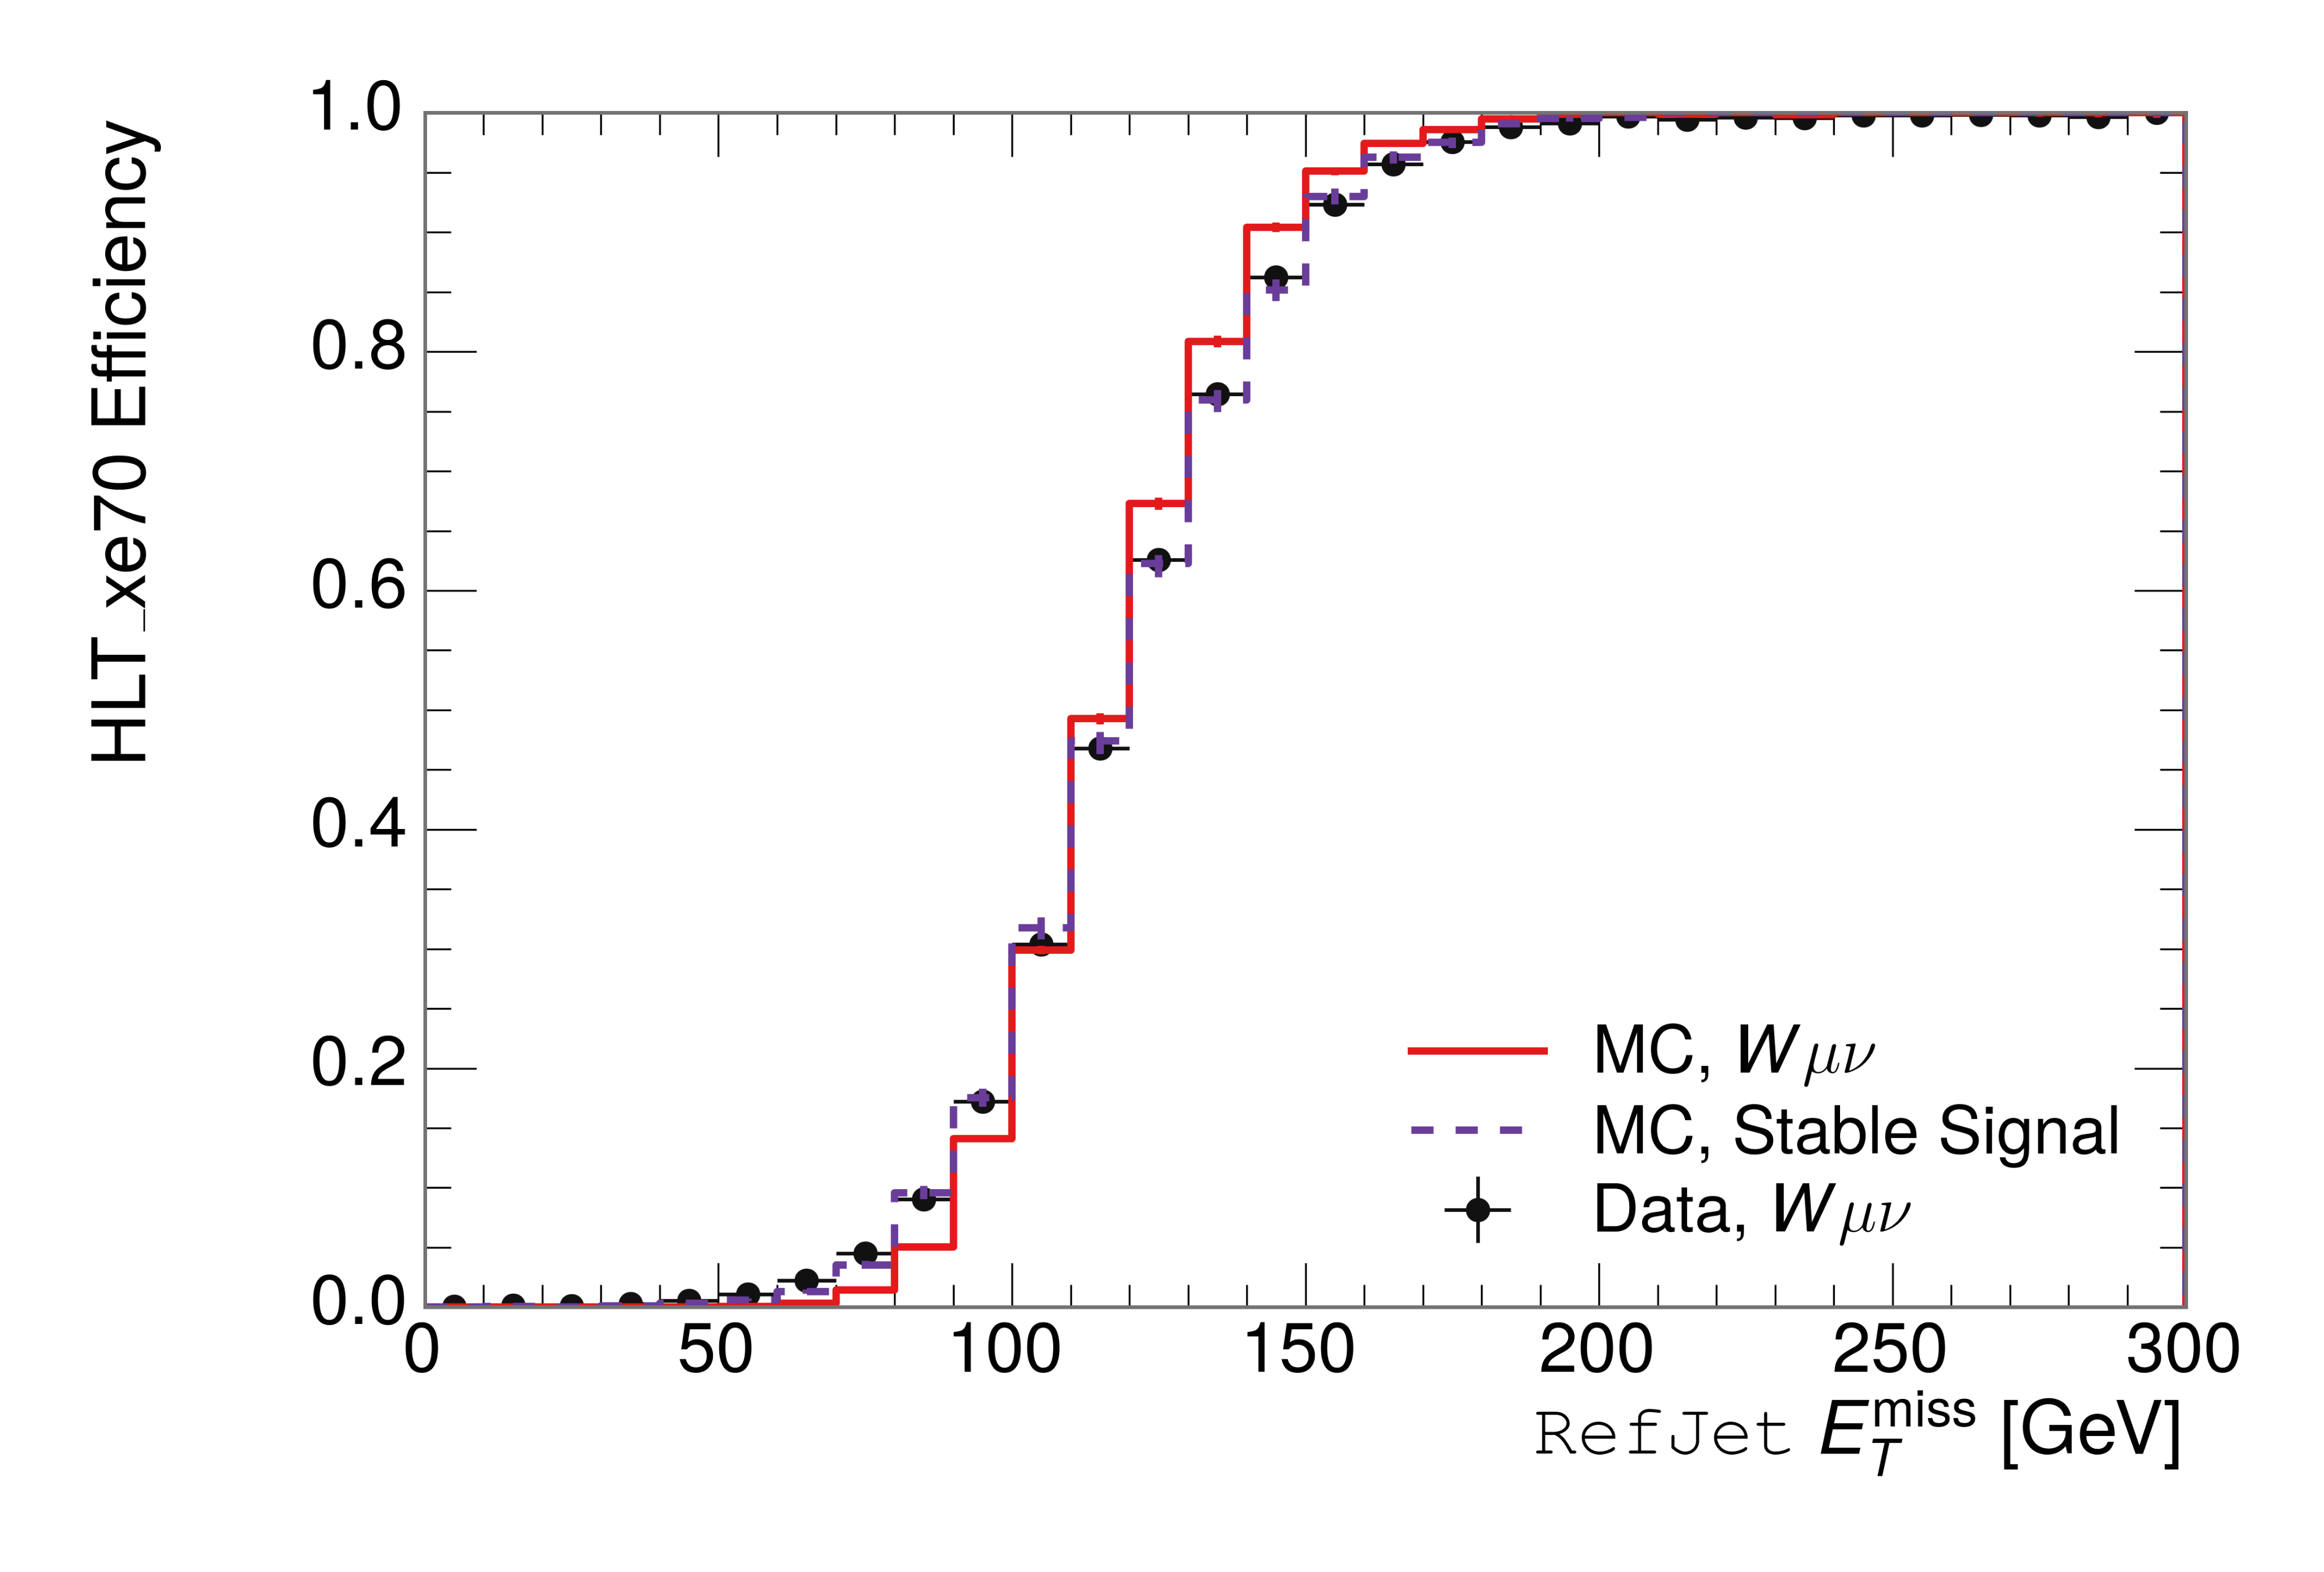
\includegraphics[width=\fullfig]{figures/hlt_xe70_calomet.png}
\caption{The trigger efficiency for the \texttt{HLT\_xe70} trigger requirement as a function of \calomet for simulated data events with a W boson selection. Simulated signal events and simulated W boson events are also included.}
\label{fig:trigger_turnon_calo}
\end{figure}

\subsubsection{Missing Transverse Momentum Scale}

The \ac{ATLAS} \ac{CP} group provides a default recommendation for systematic variations of jets and missing energy (\textbf{note: I'm not quite sure what to cite for this - I don't see any papers from the jet/met group after this was implemented}). These variations enter into this analysis only in the requirement on \met. The effect of the measured scale of \met is evaluated by varying the \met scale according to the one sigma variations provided by all \ac{CP} recommendations on objects affecting event kinematics in simulated signal events. Missing energy is reconstructed from fully reconstructed objects so any systematic uncertainties affecting jets, muons, electrons, or the \met soft terms are included. The only non-negligible contributions found using this method are itemized in Table~\ref{tab:met_syst_contributions} for an example signal sample (1200 GeV, Stable R-Hadron), where the systematic is measured as the relative difference in the final signal efficiency after applying the associated variation through the CP tools. The only variations that are significant are the grouped jet systematic variations, which combine recommended jet systematic uncertainties into linearly independent variations. 

\begin{table}
  \begin{center}
  \begin{tabular}{lcc}
  \hline
  Systematic Variation & $-$[\%]& $+$[\%] \\
  \hline
  JET\_GroupedNP\_1 & $-0.7$ & 1.3\\
  JET\_GroupedNP\_2 & $-0.7$ & 1.2\\
  JET\_GroupedNP\_3 & $-0.5$ & 1.3\\
  \hline
  \end{tabular}
  \end{center}
  \caption{Example of the contributing systematic variations to the total systematic for the \met Scale, as measured in a 1200 GeV, Stable R-Hadron signal sample.}
  \label{tab:met_syst_contributions}
\end{table}

As the peak of the reconstructed \met distribution in the signal is significantly above the current threshold for events which pass the trigger requirement, the effect of scale variation is expected to be small, which is consistent with the measured systematic of approximately 2\%. Events which do not pass the trigger requirement usually fail because there are no ISR jets in the event to balance the $R$-hadrons' transverse momentum, so the reconstructed \met is low and therefore also expected to be not very sensitive to scale changes.

\subsubsection{Momentum Parametrization}
The uncertainty on the signal efficiency from track momentum is calculated using the \ac{CP} group recommendations for tracks. 
In particular, only one recommended systematic variation affects track momentum, the sagitta bias for $q/P$. 
This uncertainty is propagated to the final selection efficiency by varying the track momentum by the recommended one sigma variation, and the associated uncertainty is found to be negligible (0.3\%). 

\subsubsection{Ionization Requirement}
The $dE/dx$ distributions in data and simulated events have different most probable values, which is due in part to radiation effects in the detector that are not fully accounted for in the simulation. 
The difference does not affect the mass measurement used in this analysis, as independent calibrations are done in simulation and in data. 
However, it does affect the efficiency of the high $dE/dx$ selection requirement. 
To calculate the size of the effect on the signal efficiency, the $dE/dx$ distribution in signal simulation is scaled by a scale factor obtained from comparing the $dE/dx$ distribution of inclusive tracks in data and in simulation. 
The difference in efficiency for this sample with a scaled $dE/dx$ distribution, relative to the nominal case, is taken as a systematic uncertainty on signal efficiency.
The uncertainty is as large as 7\% for low masses and falls to a negligible effect for large masses. 

\subsubsection{Electron and Jet Rejection}
The systematic uncertainty on the electron rejection is measured by varying the EM fraction requirement significantly, from 0.95 to 0.9. 
This is found to have a less than 0.04\% effect on signal acceptance, on average, and so is completely negligible. Similarly, the uncertainty on jet rejection is measured by tightening the \ep requirement from 0.5 to 0.4. 
This is found to have no effect on signal acceptance, so again the systematic is again negligible.

\subsubsection{Muon Veto}
The metastable signal region requires that the candidate tracks are not identified as medium muons because the majority of \rhadrons in the lifetime range included in that region do not reach the muon spectrometers before they decay. 
However, the exponential tail of the \rhadron lifetime distribution results in some \rhadrons traversing the muon spectrometer. 
These can still fail the muon medium identification because they can fail on the requirement on the number of precision hits required to pass the loose selection because they arrive late to the muon spectrometer.
This can be seen in Figure~\ref{fig:muonVeto_eff}, which shows the efficiency of the muon veto as a function of $1/\beta$, for two simulated stable \rhadron samples.

\begin{figure}[hbtp]
\centering
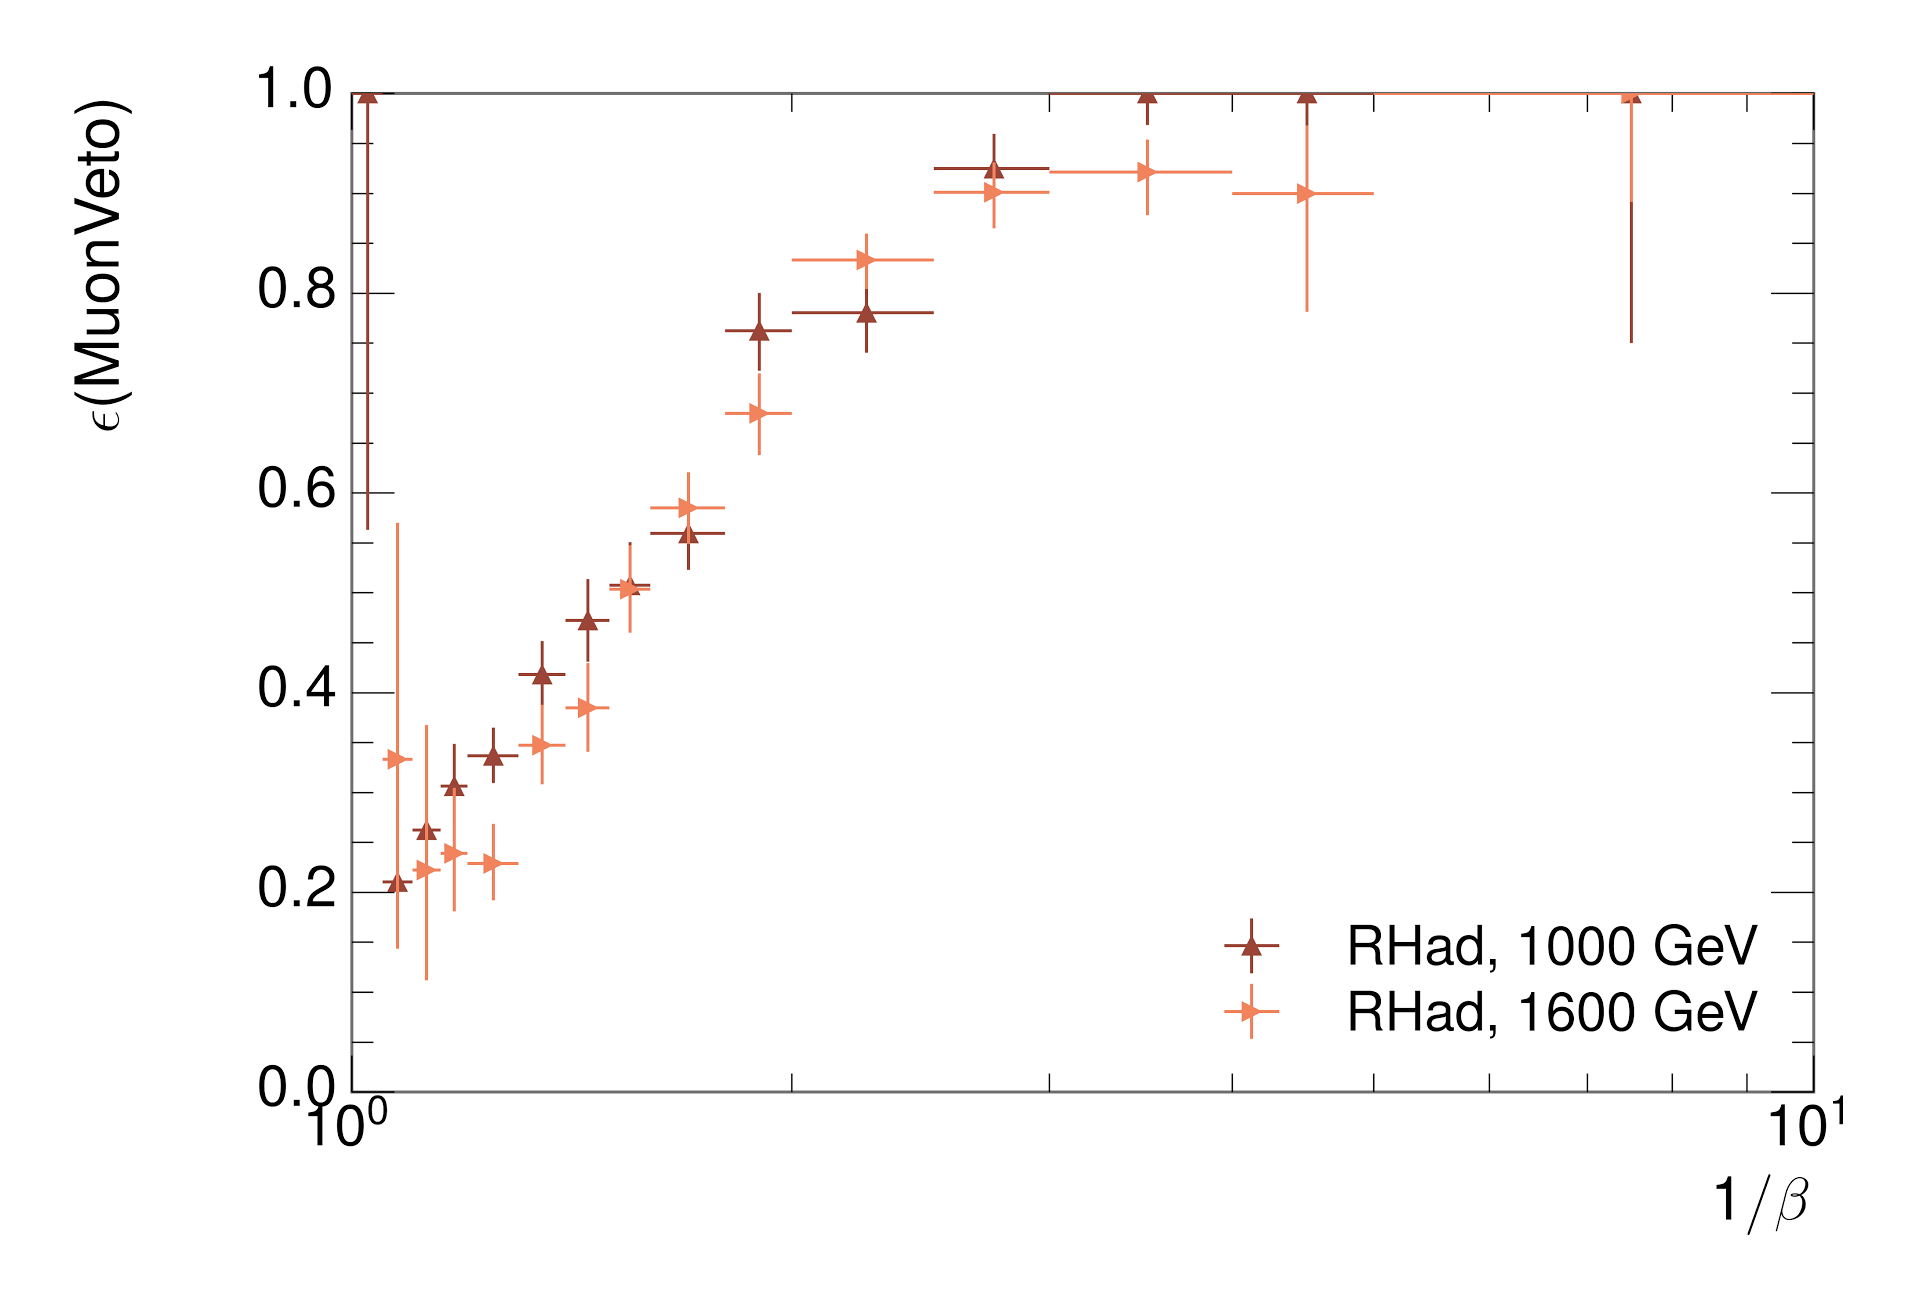
\includegraphics[width=\fullfig]{figures/veff_invbeta.png}
\caption{The efficiency of the muon veto for $R$-hadrons of two different masses, as a function of $\frac{1}{\beta}$ for simulated \rhadron tracks.}
\label{fig:muonVeto_eff}
\end{figure}

Thus, the efficiency of the muon veto depends on the timing resolution of the spectrometer, so an uncertainty is applied to the signal efficiency to cover differences in timing resolution between data and simulation. 
First, a sample of $Z\rightarrow\mu\mu$ events is selected in data in which one of the muons has a late arrival time measured in the \ac{MDT}. 
Then the reconstructed $\beta$ distribution is compared to the distribution in simulated $Z\rightarrow\mu\mu$ events; the difference between these two distributions reflects the difference in timing resolution between data and simulation.
To emulate this difference in simulated signal events, the magnitude of the difference is used to scale and shift the true $\beta$ distribution of \rhadrons in simulation. 
Signal events are then reweighted based on this varied $\beta$ distribution, and the difference in the efficiency of the muon veto selection is compared with the nominal and reweighted true $\beta$ distributions. 
The difference in muon veto efficiency is taken as a systematic uncertainty of the muon veto. 
 
The comparison of reconstructed $\beta$ between data and simulation is performed separately in the barrel, transition, and endcap regions of the spectrometer, and the reweighting of the true $\beta$ distribution in signal is done per region. 
The comparison of average reconstructed \ac{MDT} $\beta$ between data and simulation for the barrel region is shown in Figure~\ref{fig:mdt_beta} for $Z\rightarrow\mu\mu$ events.
As expected, The uncertainty is found to be negligible for $R$-hadrons with short lifetimes, and is only significant for lifetimes above 30 ns.

\begin{figure}[hbtp]
\centering
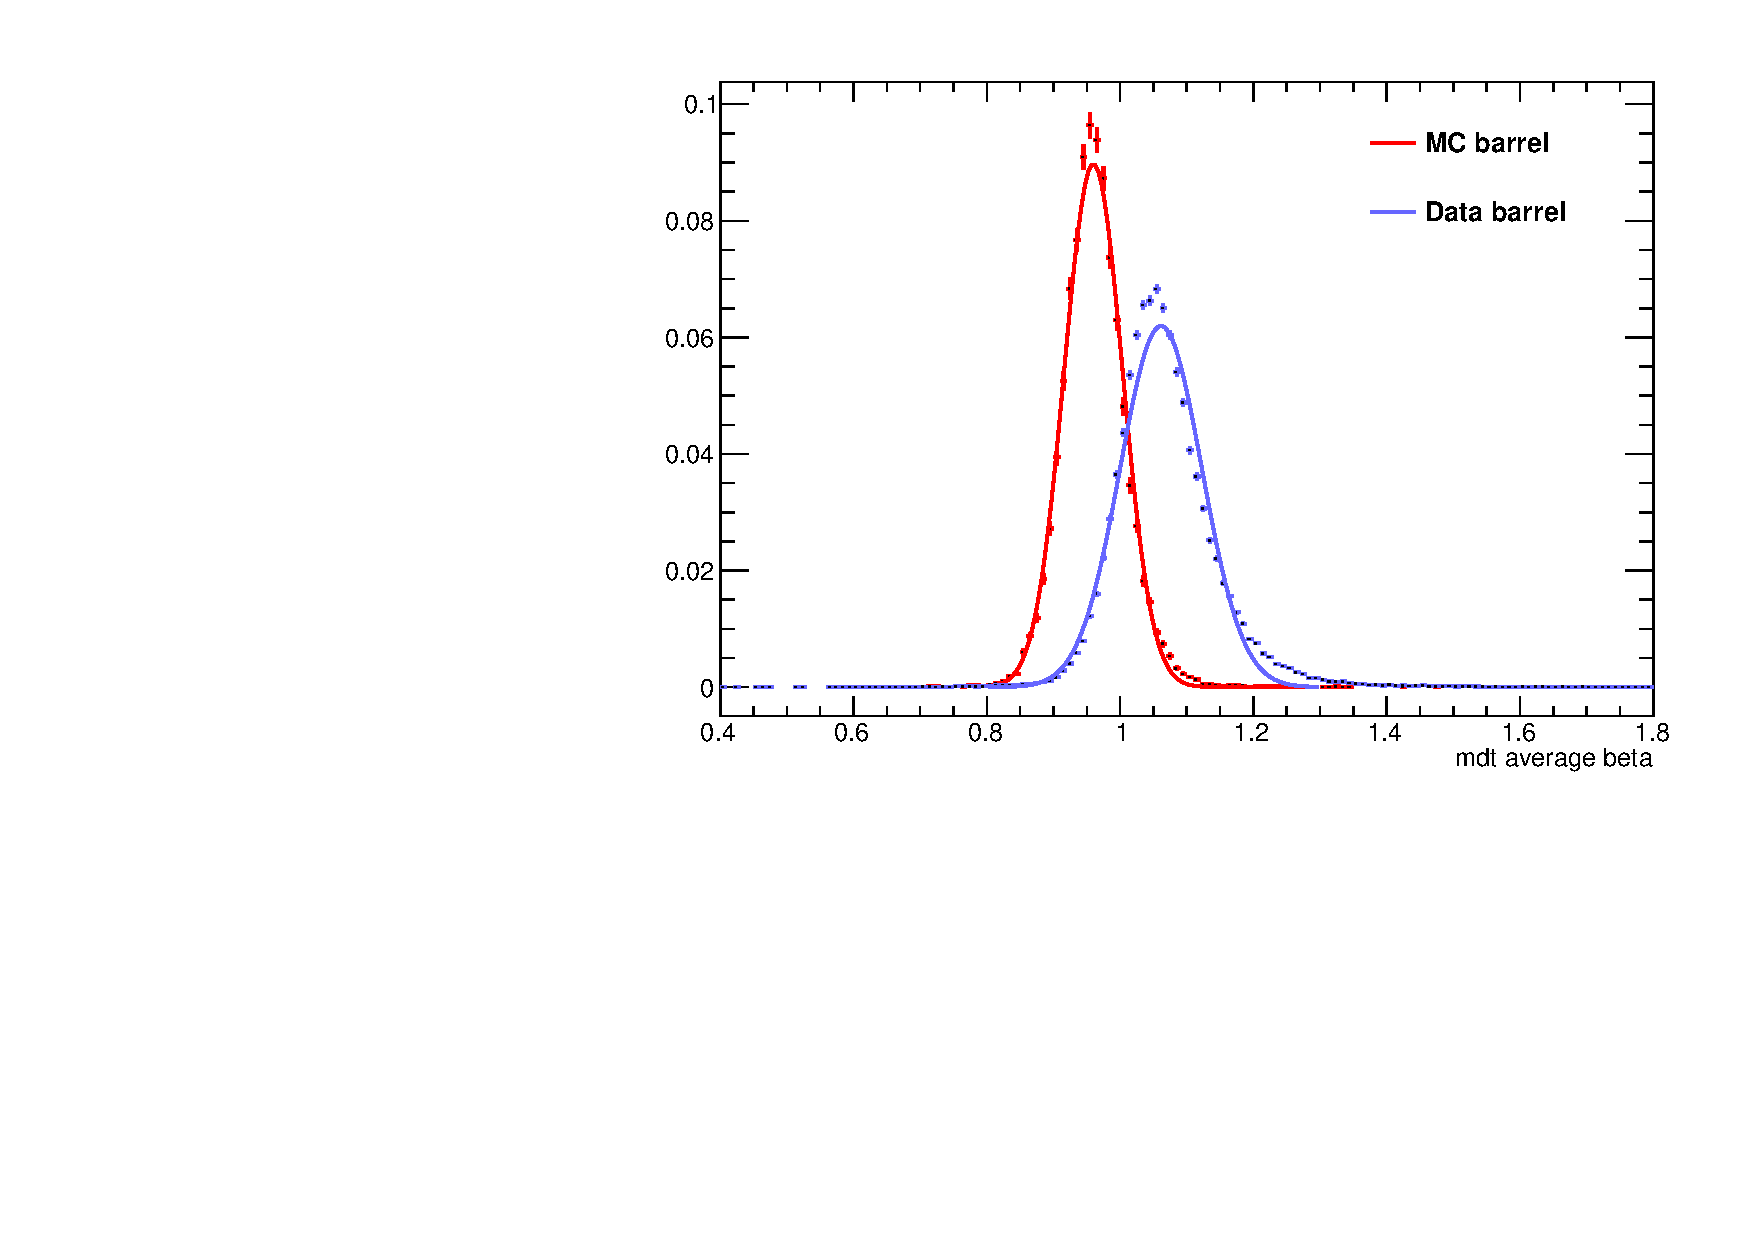
\includegraphics[width=\fullfig]{figures/beta_muonveto.pdf}
\caption{The average reconstructed MDT $\beta$ distribution for $Z\rightarrow\mu\mu$ events in which one of the muons is reconstructed as a slow muon, for both data and simulation. A gaussian fit is superimposed.}
\label{fig:mdt_beta}
\end{figure}

\subsubsection{Luminosity}
The luminosity uncertainty is provided by a luminosity measurement on \ac{ATLAS} and was measured to be 5\% at the time of the publication of this analysis.

\subsubsection{Signal Size}
As discussed in Section~\ref{sec:simulation_samples}, the signal cross sections are calculated at \ac{NLO} in the strong coupling constant with a resummation of soft-gluon emission at \ac{NLL}. 
The uncertainties on those cross sections are between 14\% to 28\% for the \rhadrons in the range of 400 to 1800 \GeV~\cite{Mackeprang:2006gx, Mackeprang:2009ad}, where the uncertainty increases with the mass.

% ----------------------------------------

\section{Final Yields}
This full analysis was performed using the 3.2 fb\tsup{-1} from the 2015 data-taking.
Using the selections discussed in Chapter~\ref{ch:selection}, sixteen events were observed in the stable signal region and eleven events were observed in the metastable signal region, prior to requirements on the candidate track mass.
The background estimate discussed in Chapter~\ref{ch:background} predicts $17 \pm 2.6 (\mathrm{stat}) \pm 1.2 (\mathrm{syst})$ events for the stable region and $11.1 \pm 1.7 (\mathrm{stat}) \pm 0.7 (\mathrm{syst})$ events for the metastable region. 
These counts are summarized in Table~\ref{tab:yields}.

\begin{table}
  \begin{center}
  \begin{tabular}{lcc}
  \hline
  Selection Region & Expected Background & Data \\
  \hline
  Stable     & $17.2 \pm 2.6 \pm 1.2$ & 16 \\
  Metastable & $11.1 \pm 1.7 \pm 0.7$ & 11 \\
  \hline
  \end{tabular}
  \end{center}
  \caption{The estimated number of background events and the number of observed events in data for the specified selection regions prior to the requirement on mass. The background estimates show statistical and systematic uncertainties.}
  \label{tab:yields}
\end{table}

The mass estimated using \dedx (Section~\ref{sec:mass_requirement}) provides the final discriminating variable, where the signal would be expected as an excess in the falling exponential tail of the expected background.
The observed distribution of masses is shown in Figure~\ref{fig:signal_mass}, along with the predicted distribution from the background estimate for each signal region.
Both include a few example simulated signal distributions, which show the scale of an excess were the \rhadron signals present.
Their is no statistically significant evidence of an excess in the data over the background estimation.
From this distribution it is clearly possible to rule out signals with lower masses, around 1200 \GeV, which have larger cross sections.

\begin{figure}
\subfloat{
  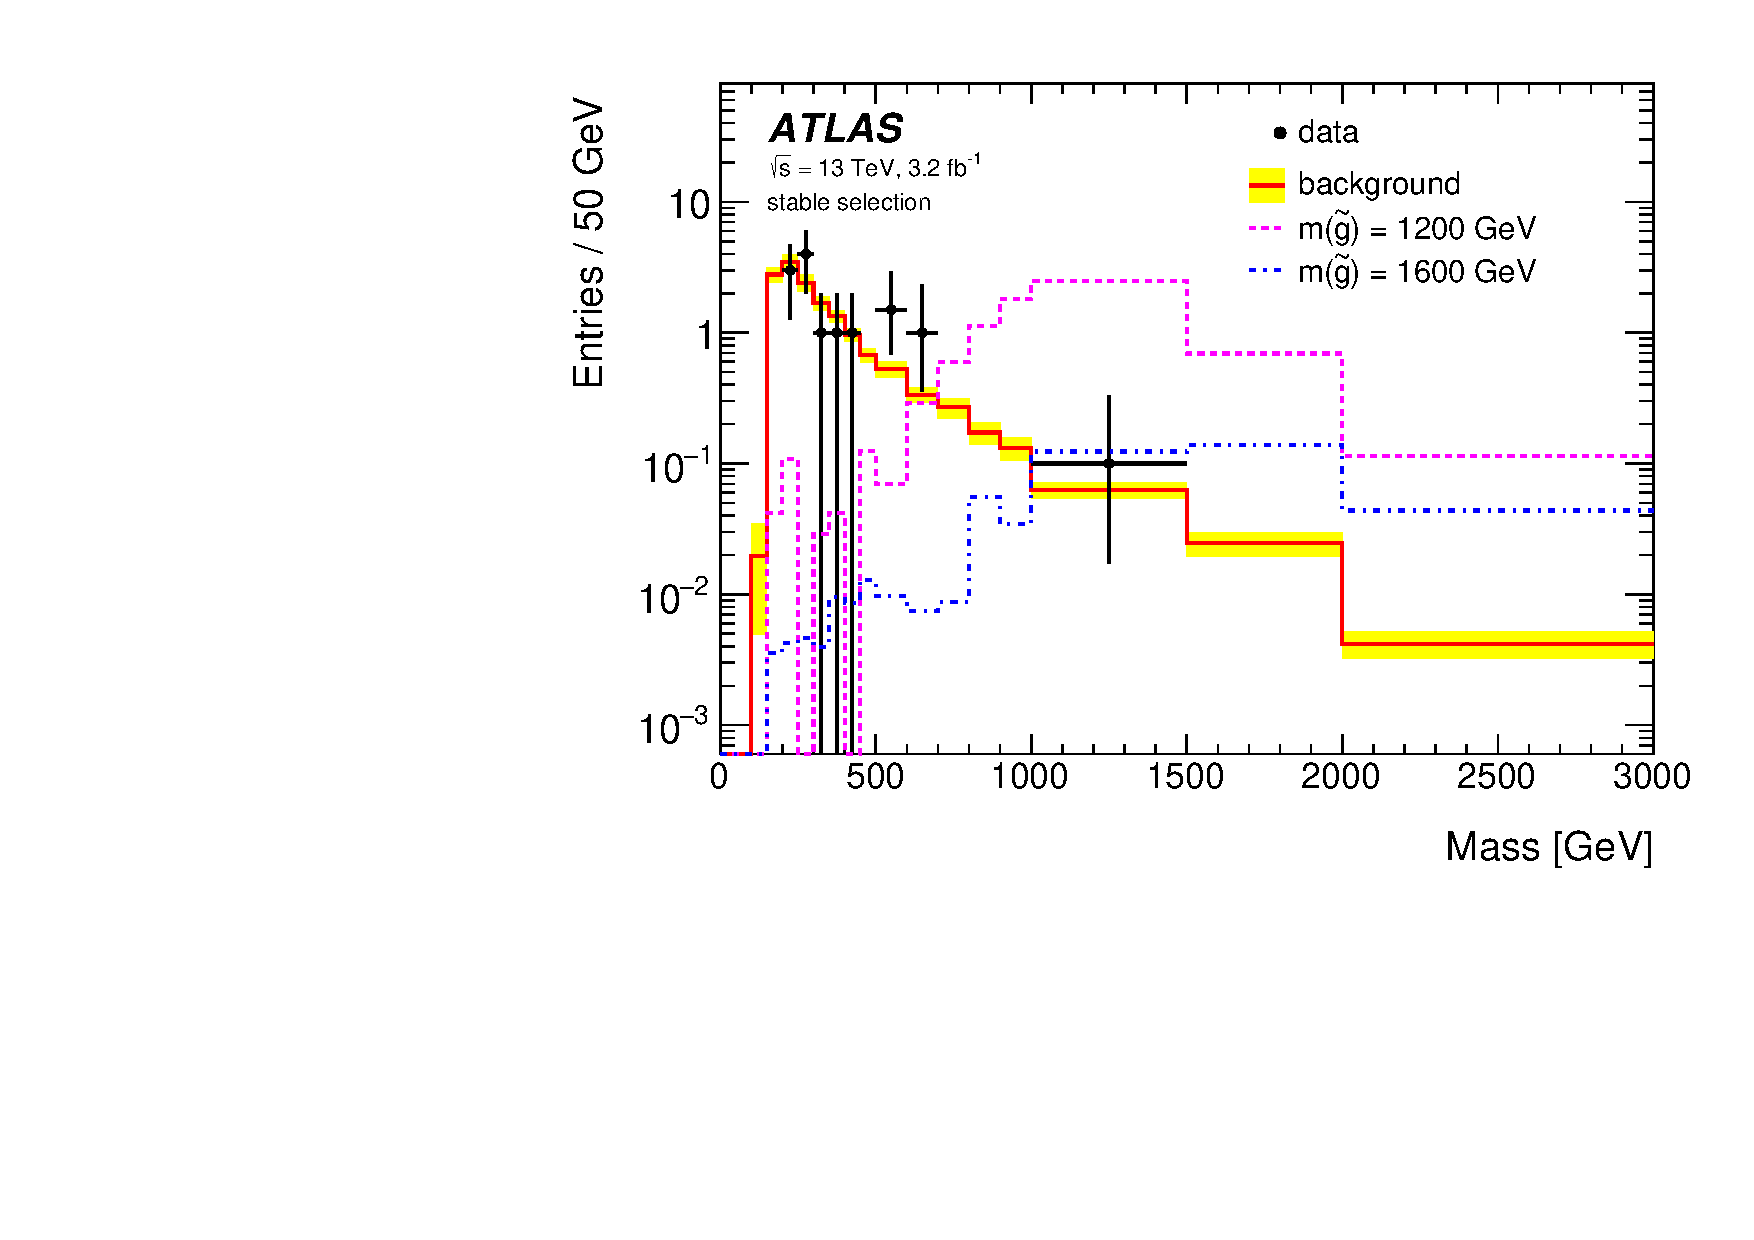
\includegraphics[width=\halffig]{figures/sr_mass_stable.pdf}
}
\subfloat{
  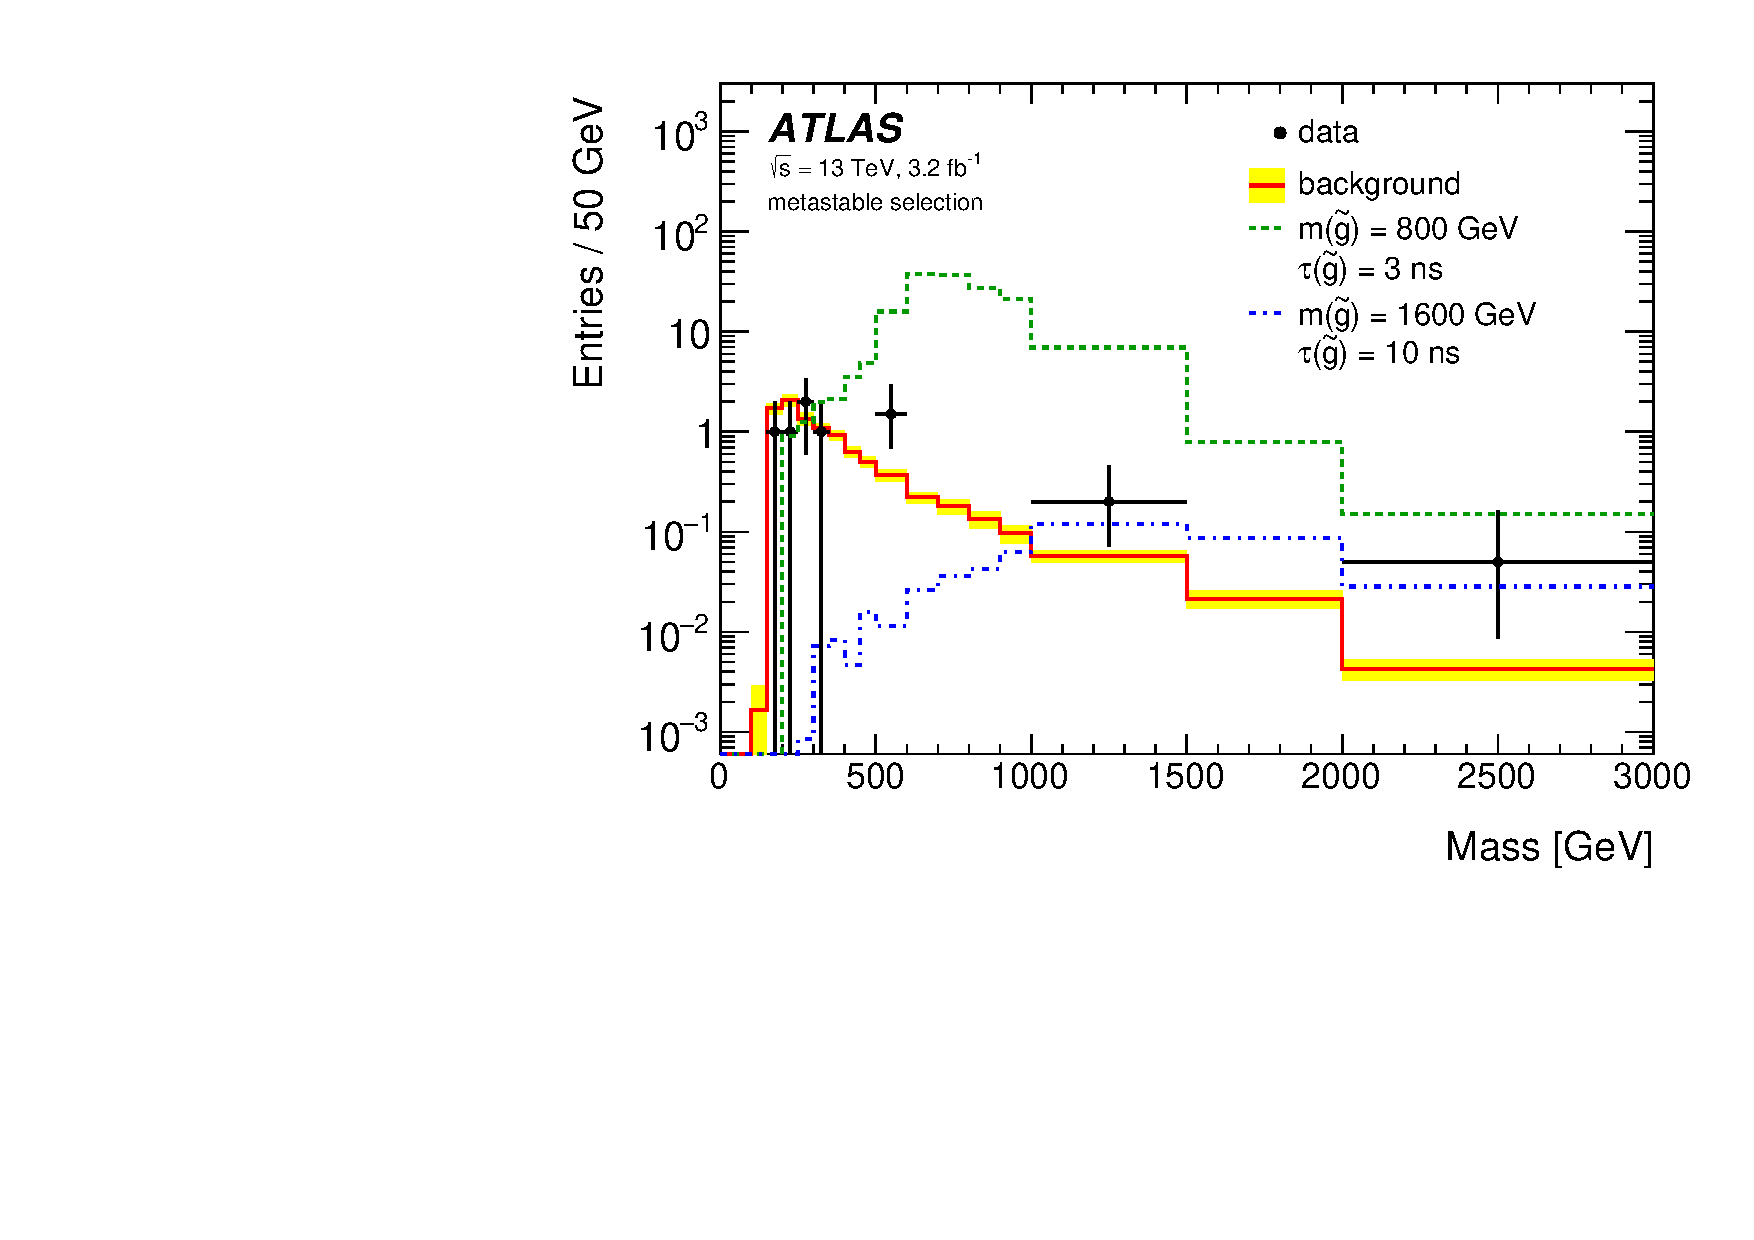
\includegraphics[width=\halffig]{figures/sr_mass_metastable.pdf}
}
\caption{The observed mass distribution of events in data and the generated background distribution in (a) the stable and (b) the metastable signal region. A few example simulated signal distributions are superimposed.}
\label{fig:signal_mass}
\end{figure}

% ----------------------------------------

\section{Cross Sectional Limits}

Because there is no observed significant excess of events in the signal region, this analysis sets upper limits on the allowed cross section for \rhadron production.
These limits are set for each mass point by counting the observed events in data, along with the expected background and simulated signal events, in windows of mass.
The mass windows are formed by fitting the distribution of signal events to a Gaussian distribution, and the window is then $\pm 1.4\sigma$ around the center of that Gaussian.
Two examples of the windows formed by this procedure are shown in Tables~\ref{tab:window_10ns}-\ref{tab:window_stable}, for the stable and 10 ns working points.
The corresponding counts of observed data, expected background, and simulated signal for those same working points are shown in Tables~\ref{tab:counts_stable}-\ref{tab:counts_10ns}.
Appendix~\ref{app:yields} includes the mass windows and counts for all of the considered signal points.

\begin{table}[!htbp]
  \begin{center}
    \begin{tabular}{ccc}
        \hline
        $m(\tilde{g})$ [GeV]  & Left Extremum [GeV] & Right Extremum [GeV] \\
        \hline
        1000    & 655 & 1349 \\
        1100    & 734 & 1455 \\
        1200    & 712 & 1631 \\
        1300    & 792 & 1737 \\
        1400    & 717 & 1926 \\
        1500    & 815 & 2117 \\
        1600    & 824 & 2122 \\
        1700    & 900 & 2274 \\
        1800    & 919 & 2344 \\
        \hline
    \end{tabular}
  \end{center}
  \caption{The left and right extremum of the mass window for each generated mass point with a 10 ns lifetime.}
  \label{tab:window_10ns}
\end{table}

\begin{table}[!htbp]
  \begin{center}
    \begin{tabular}{ccc}
        \hline
        $m(\tilde{g})$ [GeV]  & Left Extremum [GeV] & Right Extremum [GeV] \\
        \hline
        800    & 627 & 1053 \\
        1000    & 726 & 1277 \\
        1200    & 857 & 1584 \\
        1400    & 924 & 1937 \\
        1600    & 993 & 2308 \\
        1800    & 1004 & 2554 \\
        \hline
    \end{tabular}
  \end{center}
  \caption{The left and right extremum of the mass window used for each generated stable mass point.}
  \label{tab:window_stable}
\end{table}

\begin{table}[!htbp]
  \begin{center}
    \begin{tabular}{c|c|c|c}
      \hline
      $m(\tilde{g})$ [GeV]  & Expected Signal & Expected Background & Observed Data\\
      \hline
      800    & $462.83 \pm 14.86 $ & $1.764 \pm 0.080 $ & $2.0$ \\
      1000   & $108.73 \pm 3.38 $  & $1.458 \pm 0.070 $ & $1.0$ \\
      1200   & $31.74 \pm 0.95 $   & $1.137 \pm 0.060 $ & $1.0$ \\
      1400   & $10.22 \pm 0.29 $   & $1.058 \pm 0.058 $ & $1.0$ \\
      1600   & $3.07 \pm 0.09 $    & $0.947 \pm 0.054 $ & $1.0$ \\
      1800   & $1.08 \pm 0.05 $    & $0.940 \pm 0.054 $ & $1.0$ \\
      \hline
    \end{tabular}
  \end{center} 
  \caption{The expected number of signal events, the expected number of background events, and the observed number of events in data with their respective statistical errors within the respective mass window for each generated stable mass point}
  \label{tab:counts_stable}
\end{table}

\begin{table}[!htbp]
  \begin{center}
    \begin{tabular}{cccc}
      \hline
      $m(\tilde{g})$ [GeV]  & Expected Signal & Expected Background & Observed Data\\ 
      \hline
      1000    & $144.48 \pm 5.14 $ & $1.499 \pm 0.069 $ & $2.0$ \\
      1100    & $73.19 \pm 2.61 $  & $1.260 \pm 0.060 $ & $2.0$ \\
      1200    & $41.54 \pm 1.41 $  & $1.456 \pm 0.067 $ & $2.0$ \\
      1300    & $22.58 \pm 0.77 $  & $1.201 \pm 0.058 $ & $2.0$ \\
      1400    & $12.70 \pm 0.42 $  & $1.558 \pm 0.071 $ & $2.0$ \\
      1500    & $6.73 \pm 0.24 $   & $1.237 \pm 0.060 $ & $2.0$ \\
      1600    & $3.90 \pm 0.13 $   & $1.201 \pm 0.058 $ & $2.0$ \\
      1700    & $2.27 \pm 0.07 $   & $1.027 \pm 0.052 $ & $2.0$ \\
      1800    & $1.34 \pm 0.04 $   & $1.019 \pm 0.052 $ & $2.0$ \\
      \hline
    \end{tabular}
  \end{center}
  \caption{The expected number of signal events, the expected number of background events, and the observed number of events in data with their respective statistical errors within the respective mass window for each generated mass point with a lifetime of 10 ns.}
  \label{tab:counts_10ns}
\end{table}


The 95\% confidence level upper limits on the cross sections for a large grid of masses (between 800 and 1800 \GeV) and lifetimes (between 0.4 and stable) are extracted from these counts with the $CL_{S}$ method using the profile likelihood ratio as a test statistic~\cite{CLS_method}.
For this procedure, the systematic uncertainties estimated for the signal and background yields are treated as Gaussian-distributed nuissance parameters.
The uncertainty on the normalization of the expected background distribution is included in the expected background events.
At this point the expected cross section limit is calculated for both the metastable and stable signal region for each lifetime point, and the region with the best expected limit is selected for each lifetime.
Using that procedure, the metastable region is used for lifetimes up to and including 30 ns, and the stable region for lifetimes above it. 


The resulting cross-sectional upper limits are shown as a function of mass in Figure~\ref{fig:xsec_limit_stable} and Figure~\ref{fig:xsec_limit_metastable} for each lifetime considered.
The limits are interpolated linearly between each mass point, and the dependence of the limit on the mass is small as the efficiency is relatively constant for large \rhadron masses.
There is however a strong dependence on lifetime, as discussed in Section~\ref{sec:efficiency}, where the probability to form a fully reconstructed track and the kinematic freedom to produce \met result in a local maximum in the limit at 10-30 ns.
The figures also include the expected cross section for pair-produced gluino \rhadrons for reference.
For the 10 ns and stable cross section limits, both the observed limit and expected cross section for the Run 1, 8 \TeV version of this analysis are included.
There the cross sectional limits are lower because of the increased available luminosity, while the signal cross sections were also much lower because of the lower collision energy.

\begin{figure}
\centering
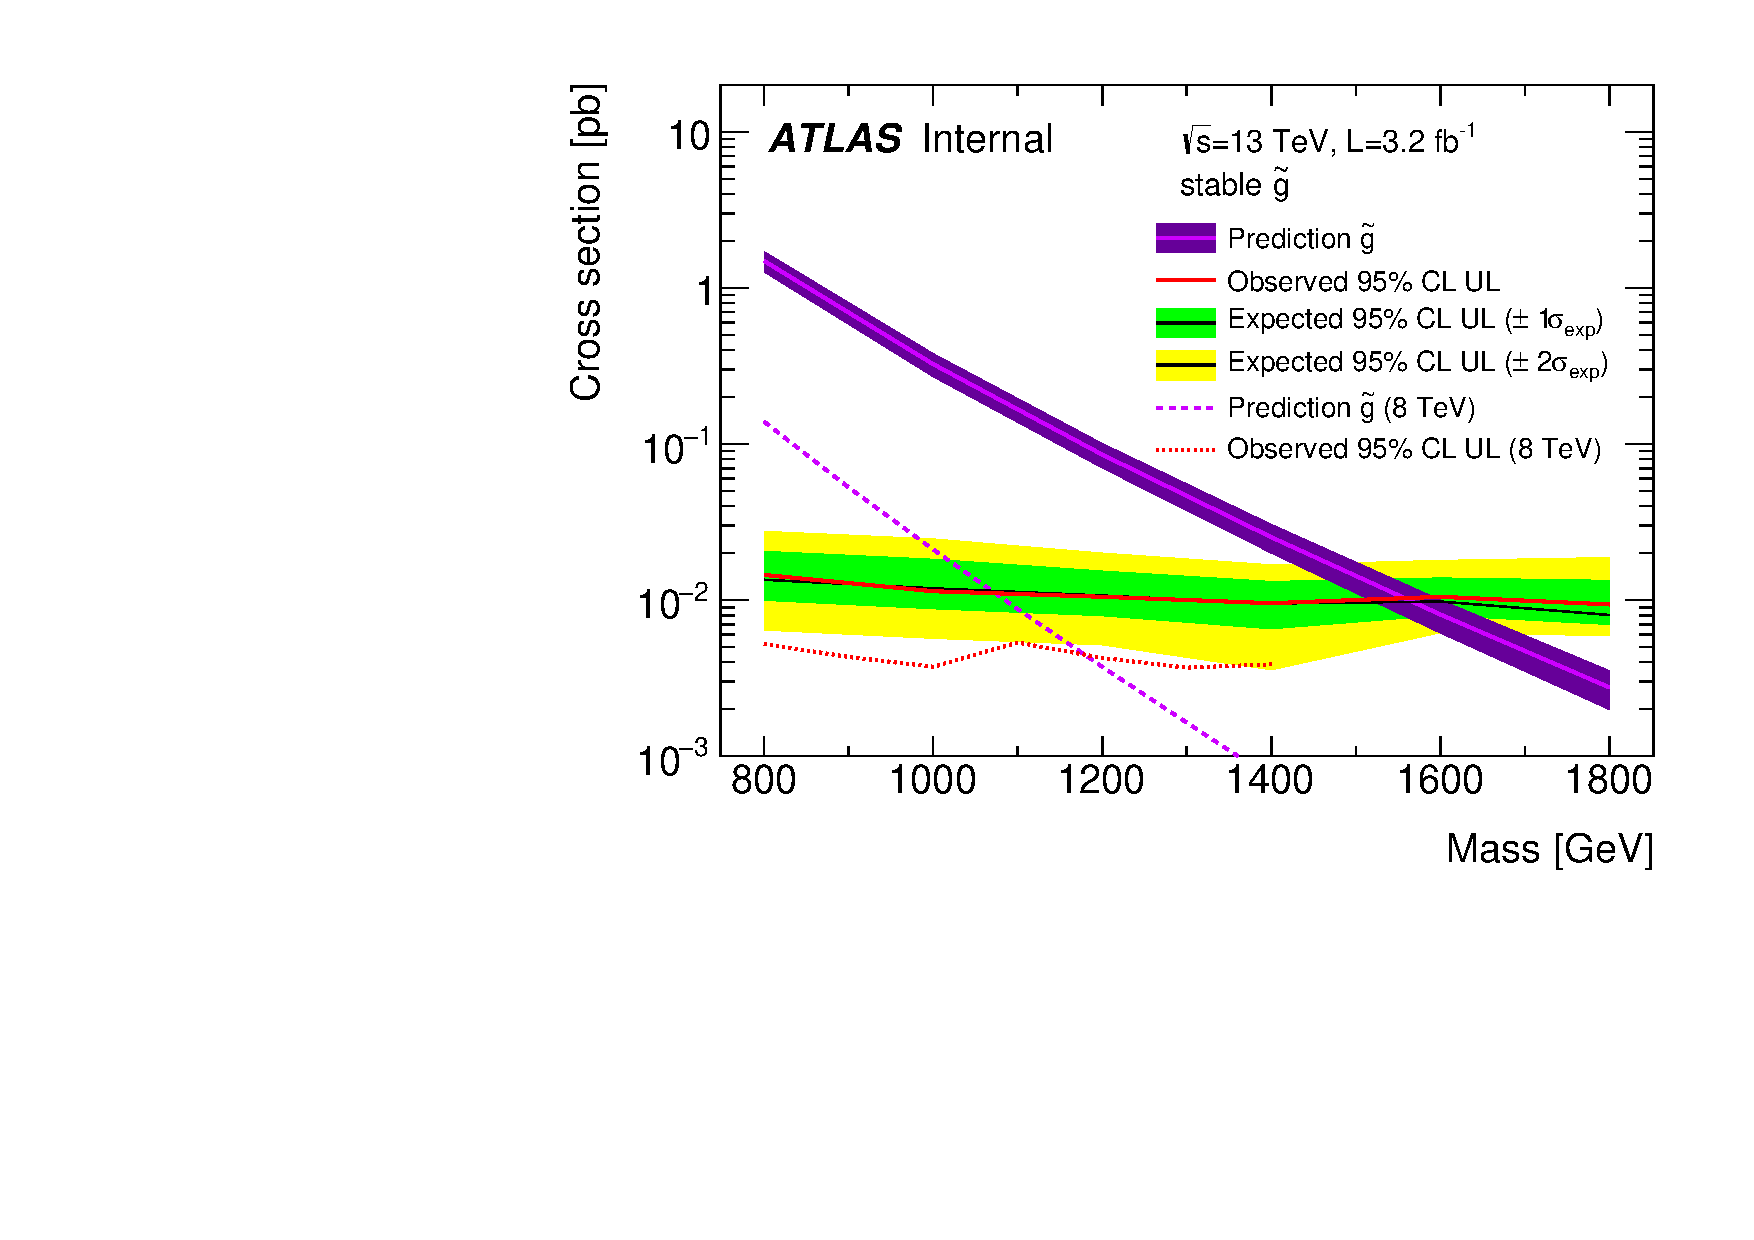
\includegraphics[width=\fullfig]{figures/xsec_limit_stable.pdf}
\caption{The observed and expected cross section limits as a function of mass for the stable simulated signal. The predicted cross section values for the corresponding signals are included.}
\label{fig:xsec_limit_stable}
\end{figure}

\begin{figure}
\subfloat{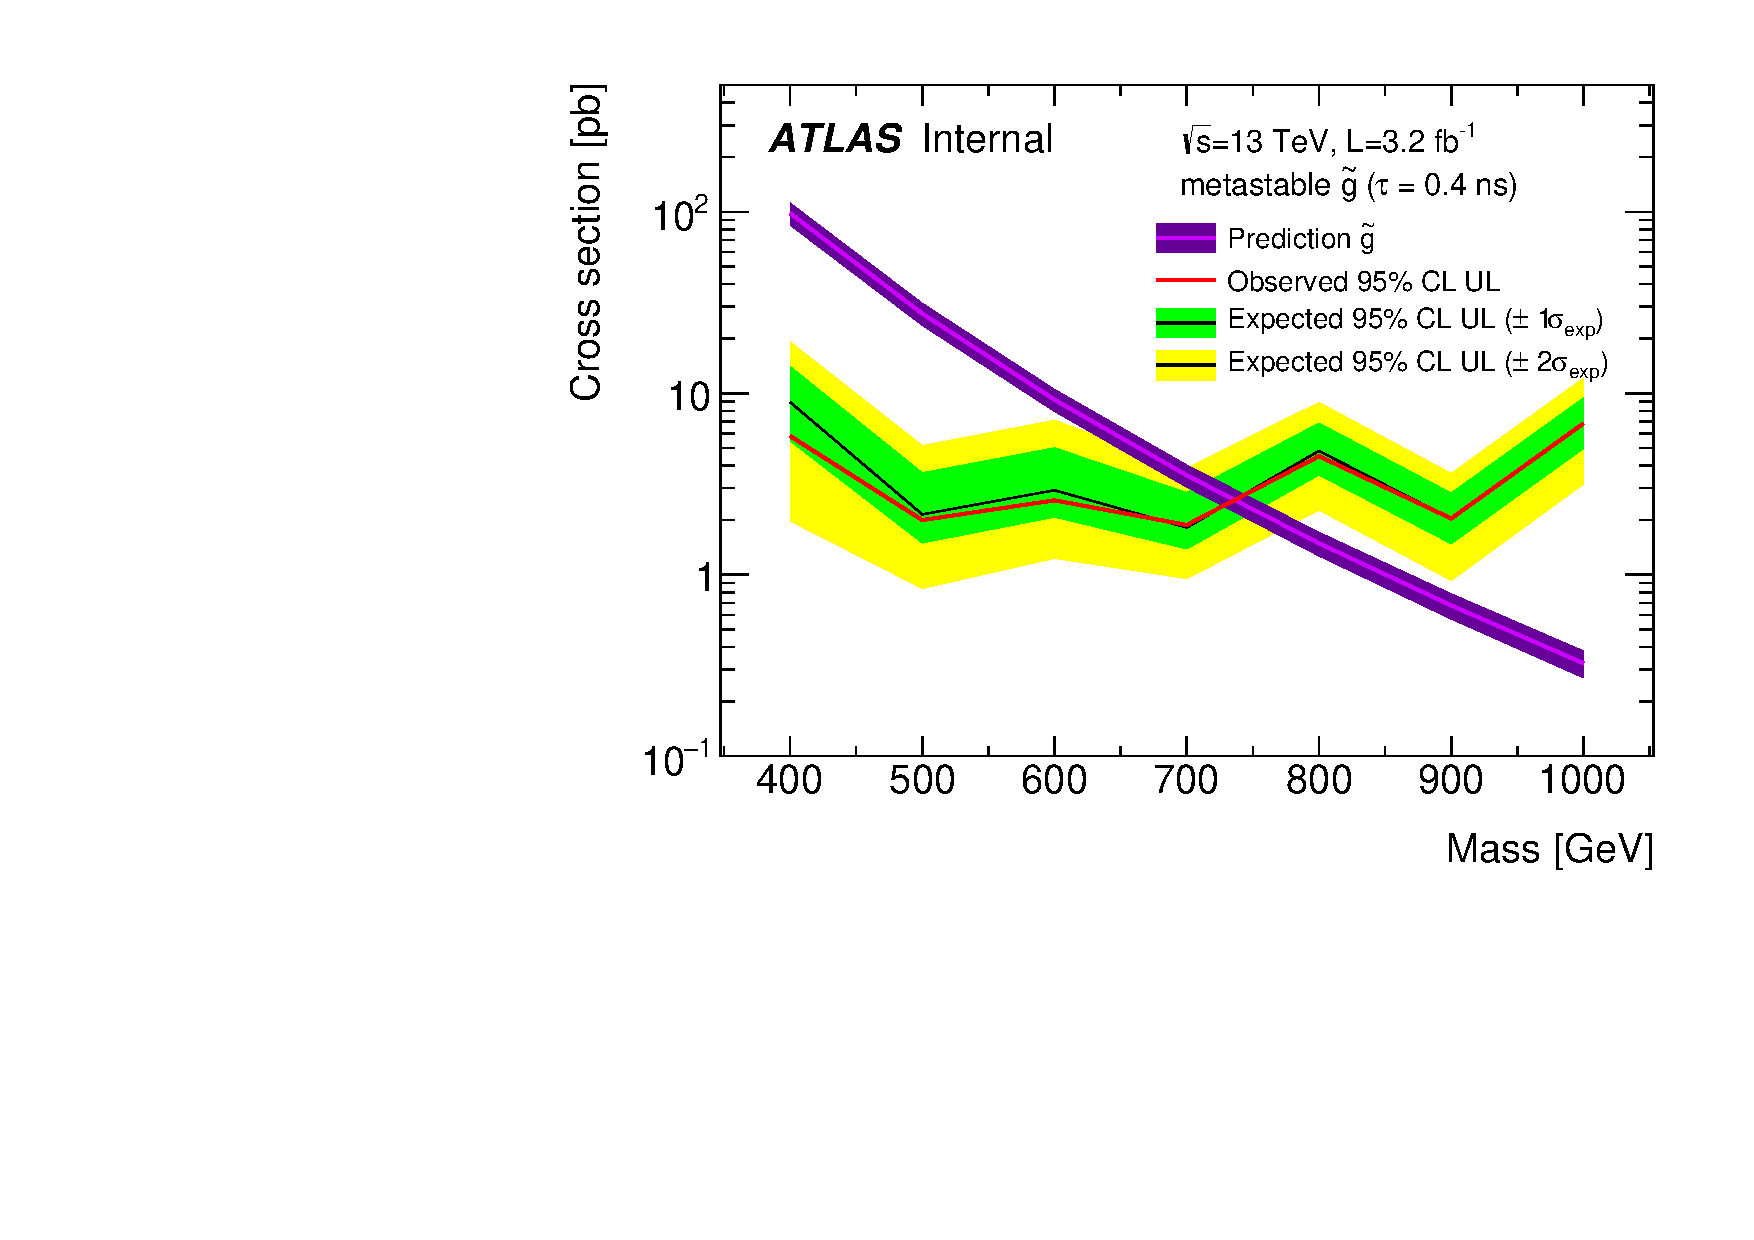
\includegraphics[width=\halffig]{figures/xsec_limit_p4ns.pdf}}
\subfloat{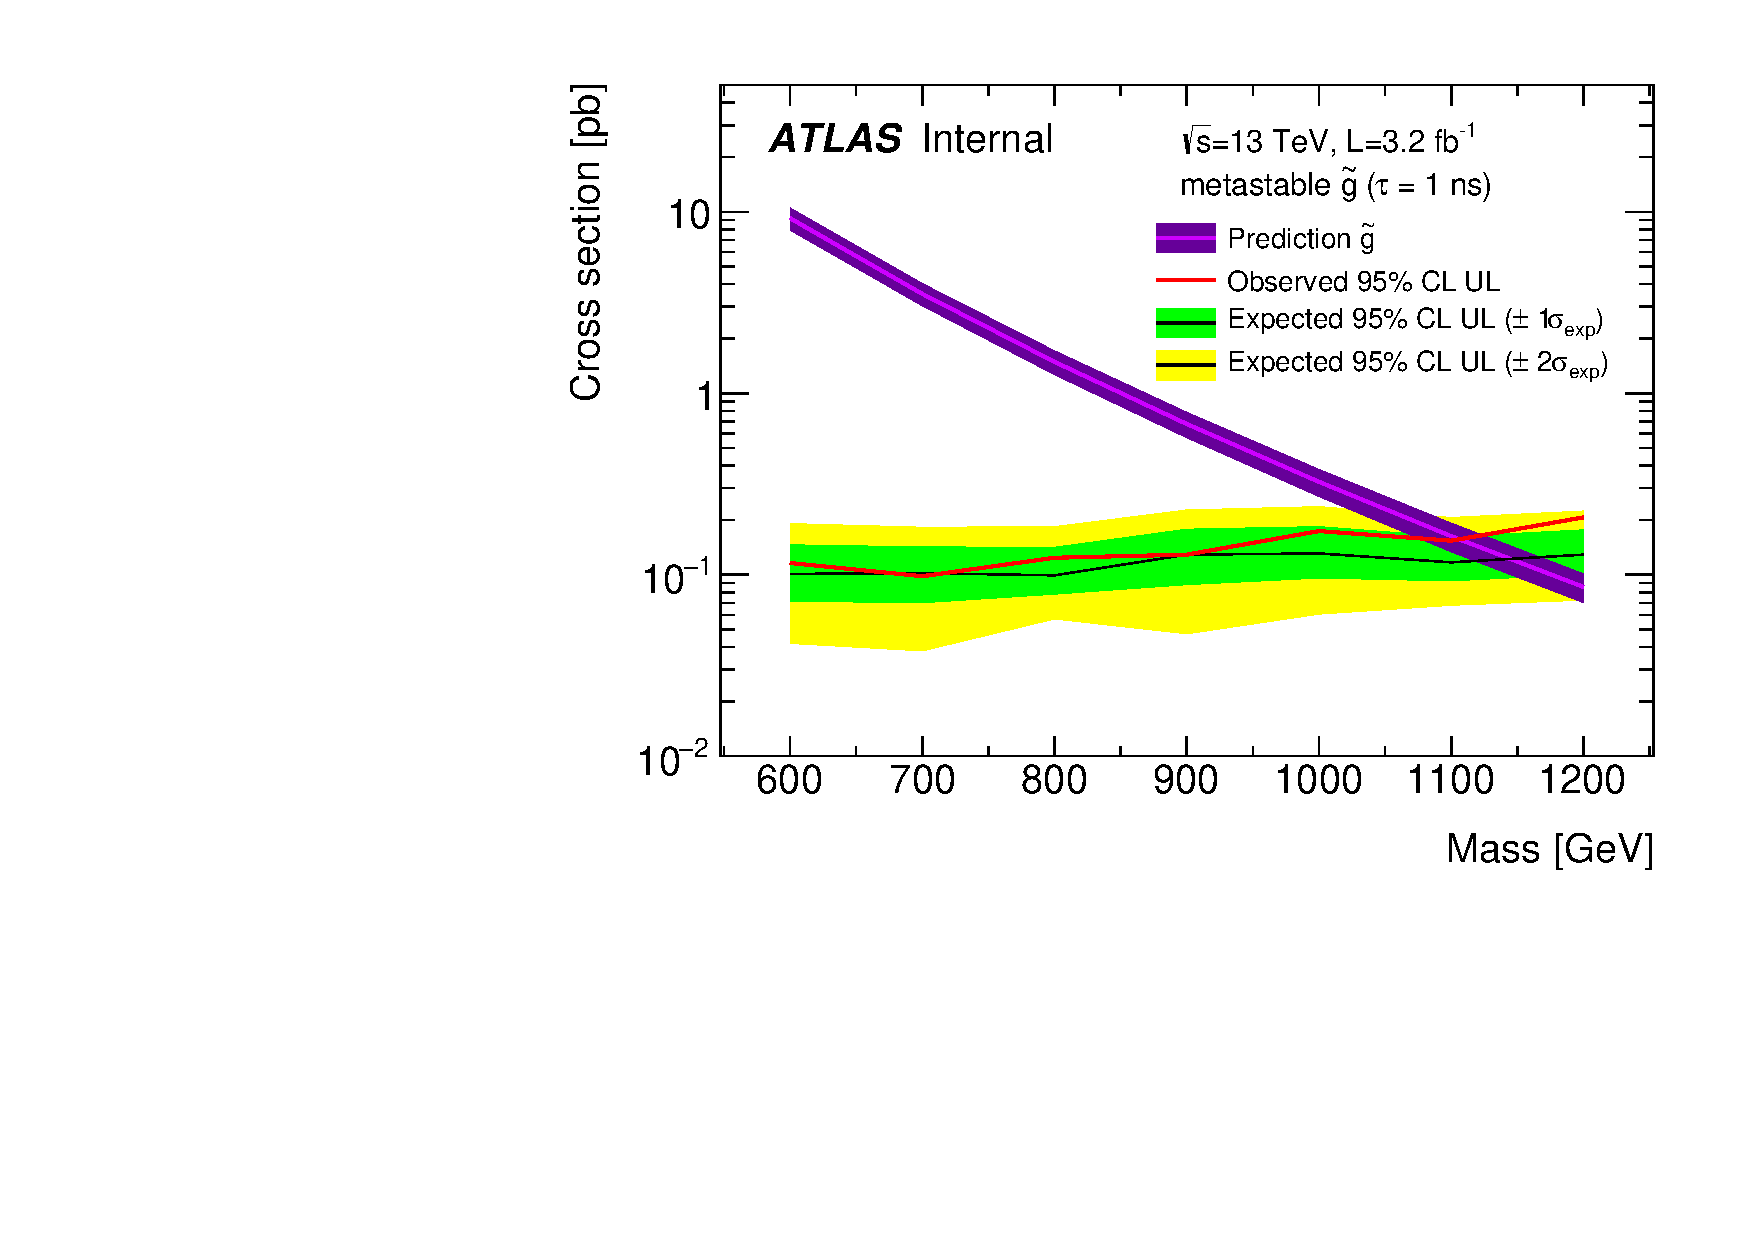
\includegraphics[width=\halffig]{figures/xsec_limit_1ns.pdf}}\\
\subfloat{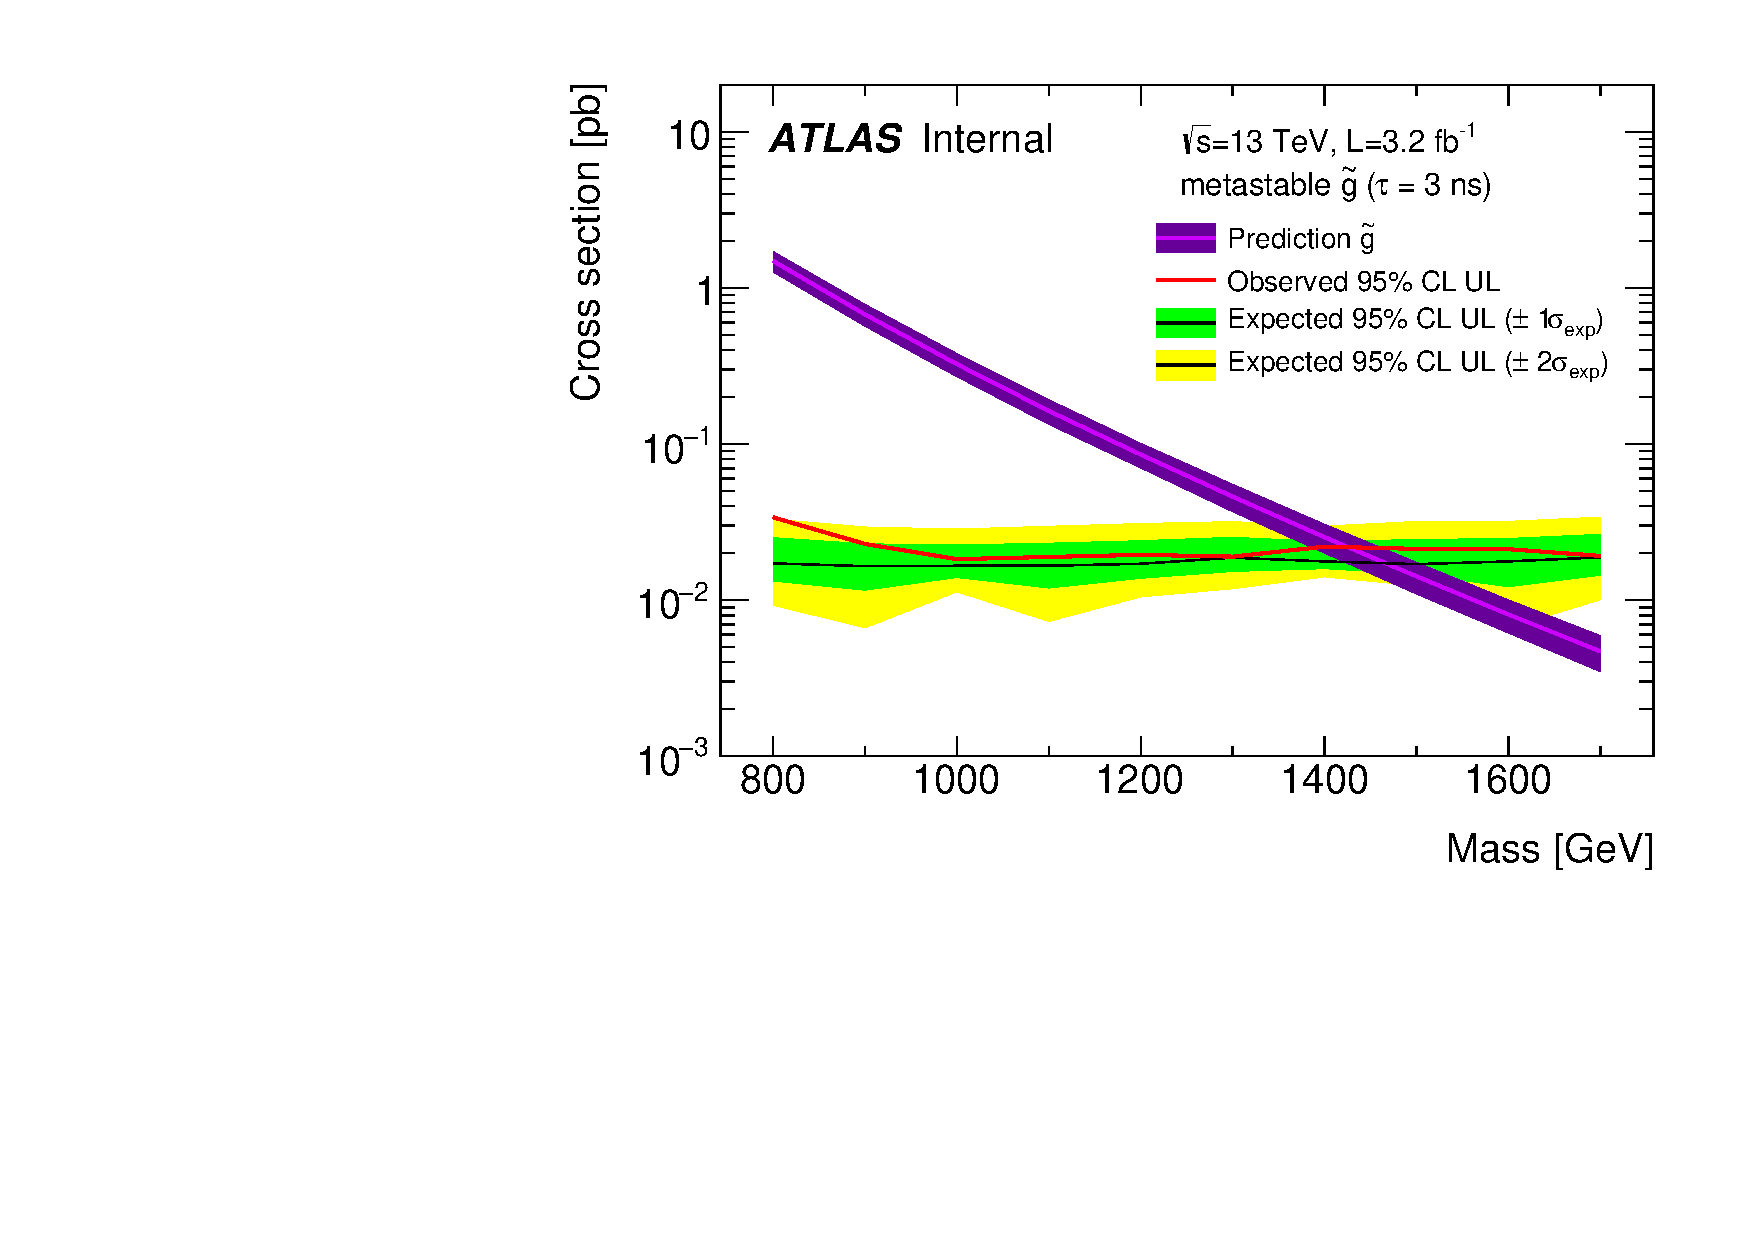
\includegraphics[width=\halffig]{figures/xsec_limit_3ns.pdf}}
\subfloat{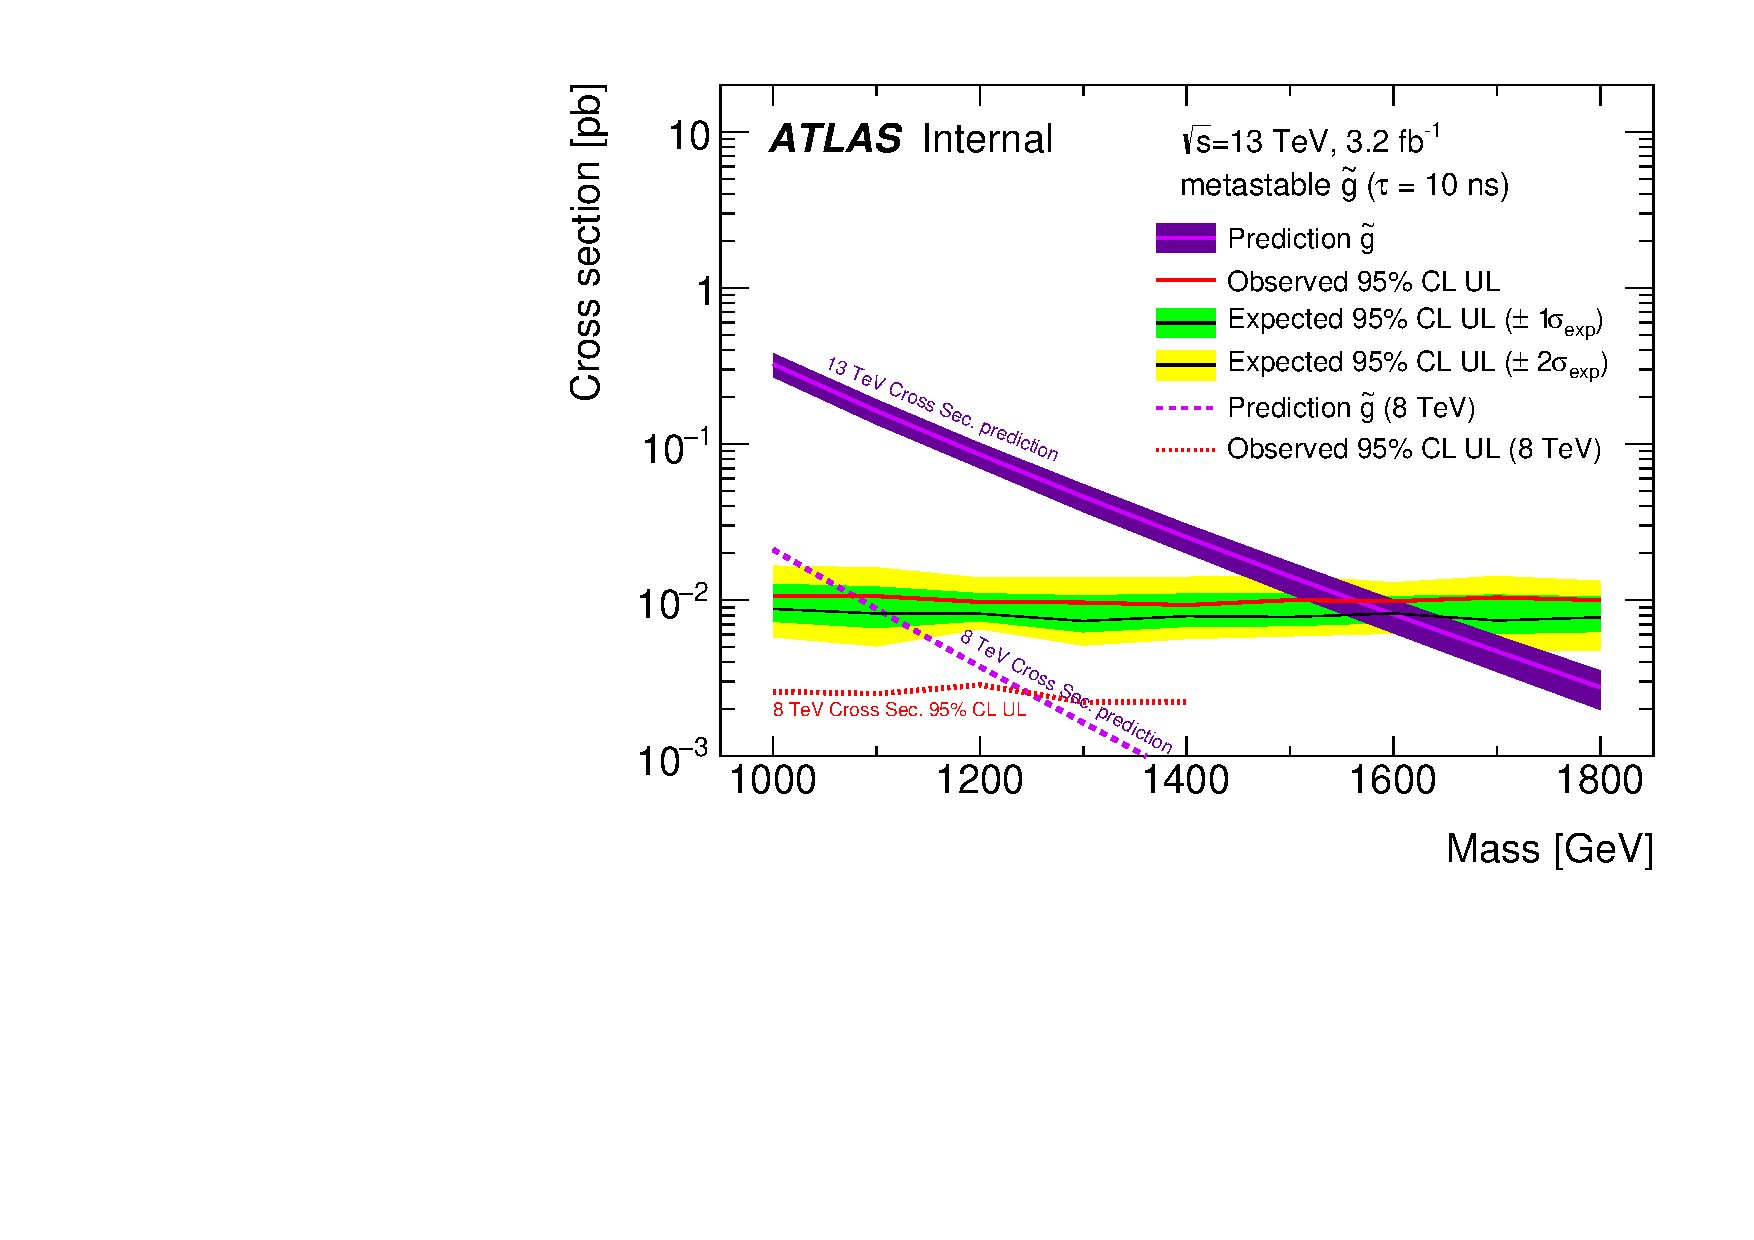
\includegraphics[width=\halffig]{figures/xsec_limit_10ns.pdf}}\\
\subfloat{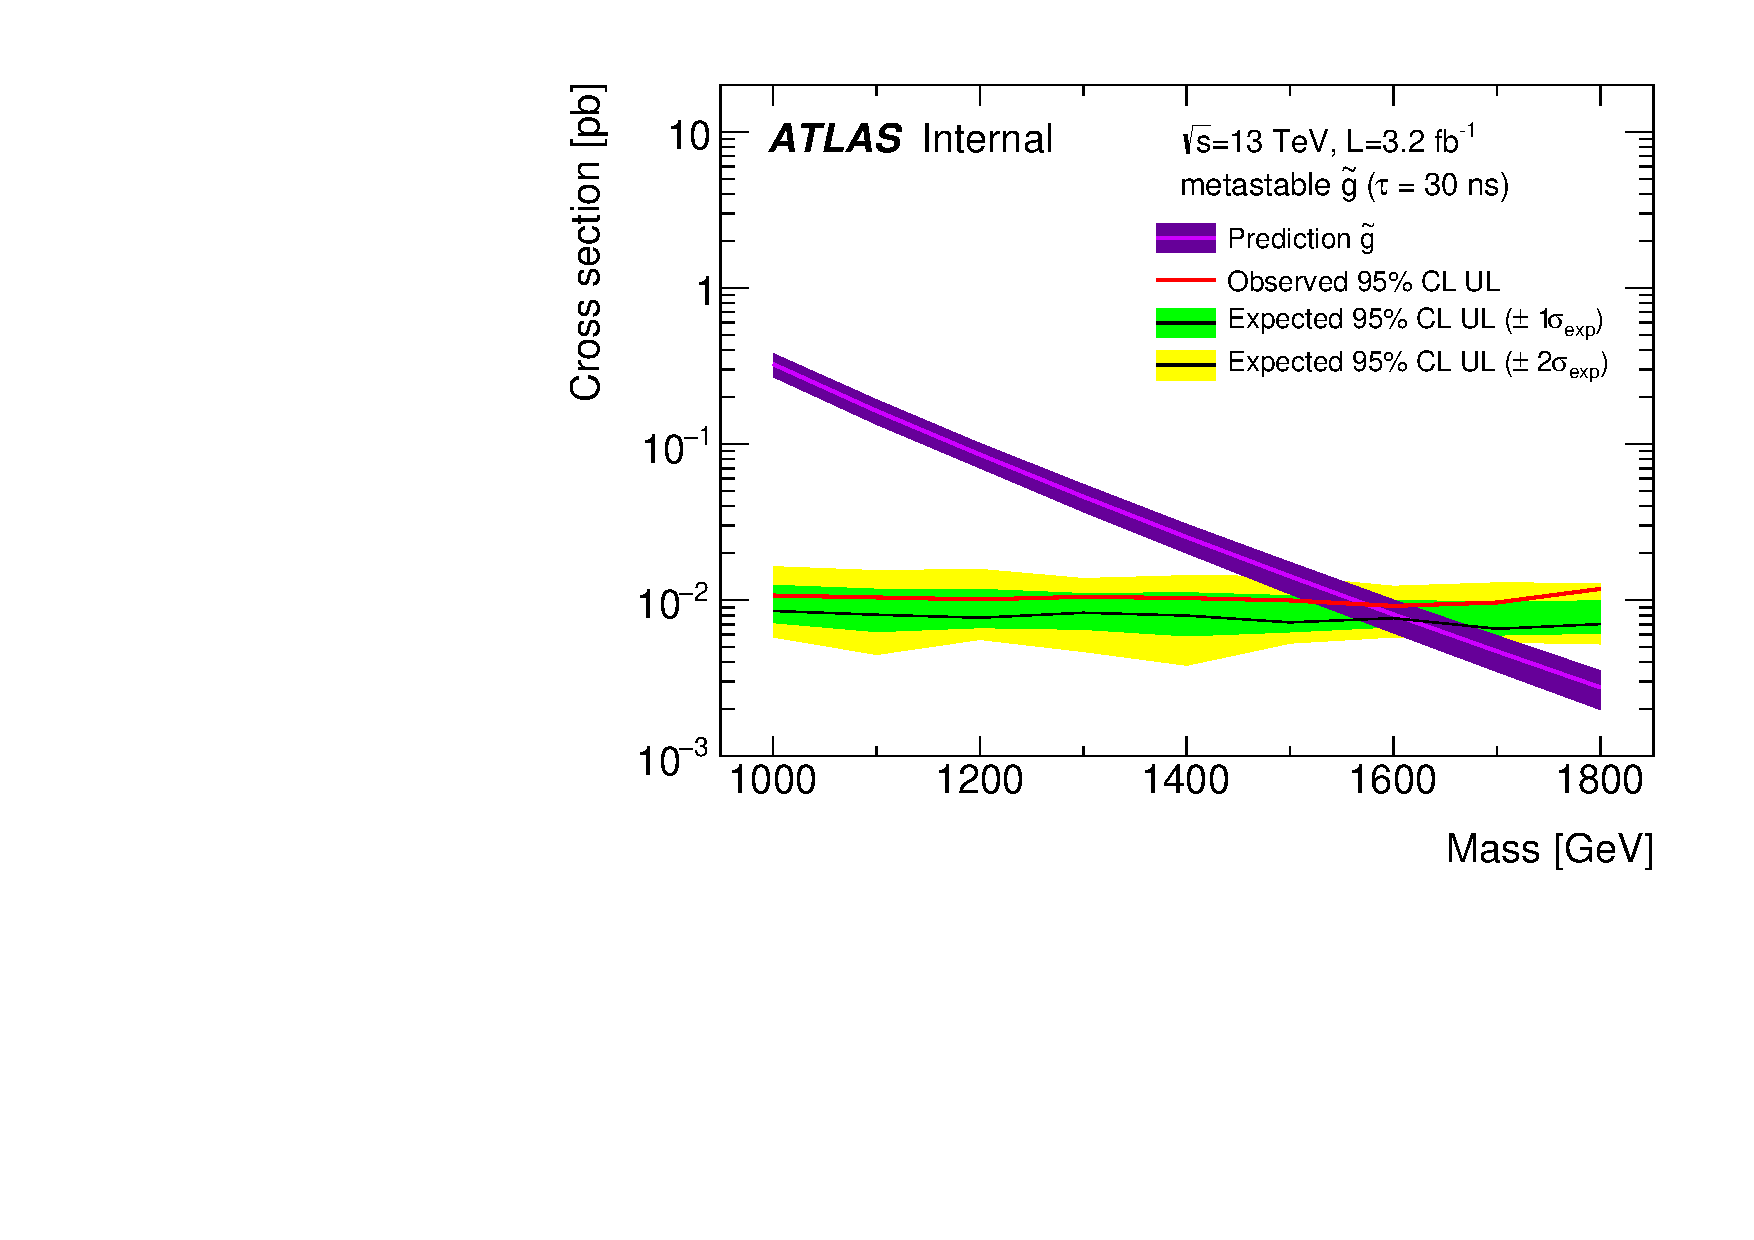
\includegraphics[width=\halffig]{figures/xsec_limit_30ns.pdf}}
\subfloat{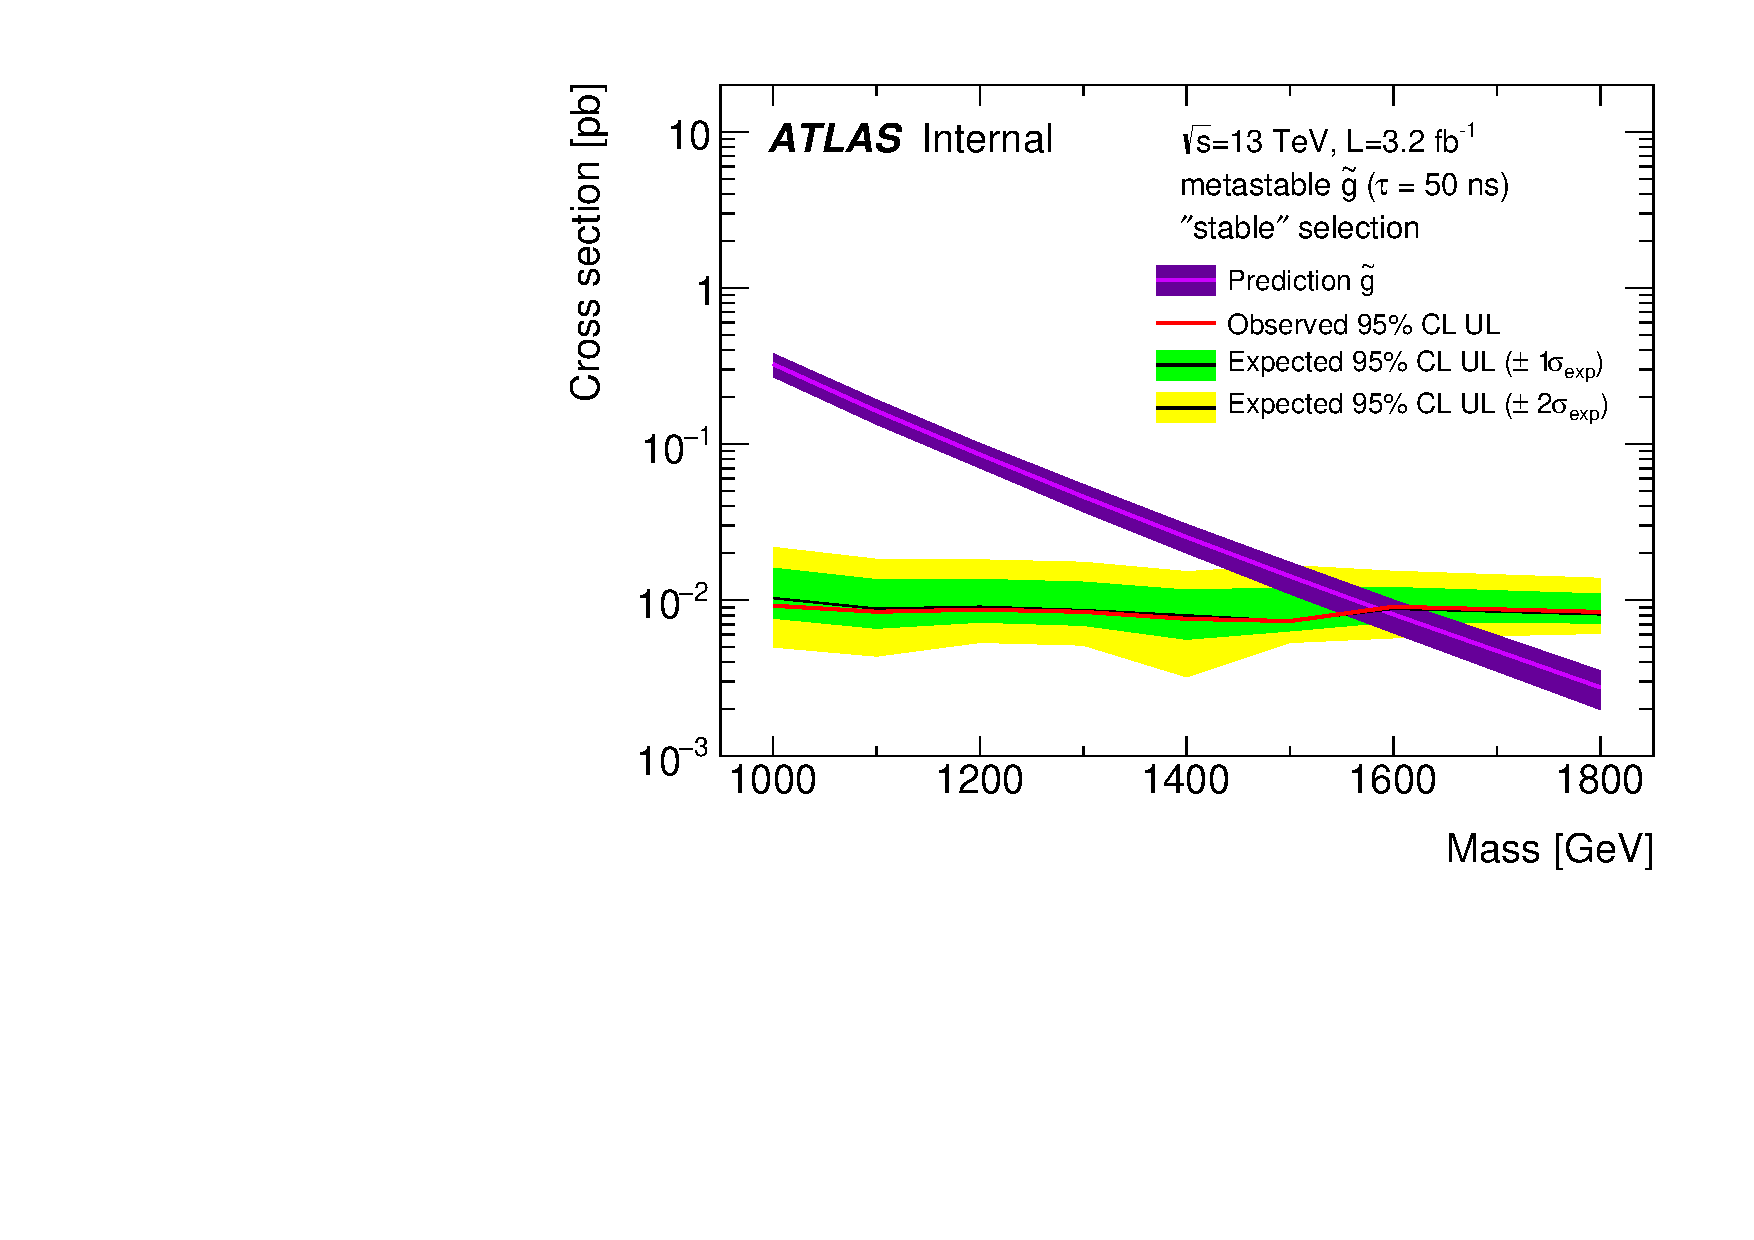
\includegraphics[width=\halffig]{figures/xsec_limit_50ns.pdf}}\\
\caption{The observed and expected cross section limits as a function of mass for each generated lifetime. The predicted cross section values for the corresponding signals are included.}
\label{fig:xsec_limit_metastable}
\end{figure}



% ----------------------------------------

\section{Mass Limits}

The cross-sectional limits can then be used to derive a lower mass limit for gluino \rhadrons by comparing them to the theoretically predicted production cross sections.
These mass limits range from only 740 \GeV at the lowest lifetimes considered, where the selection efficiency is very low, to up to 1580 \GeV at 30 ns where the selection efficiency is maximized.
The observed and expected mass limits for each lifetime point are detailed in Table~\ref{tab:mass_limits}, which also lists which selection region was used for each lifetime.
These excluded range of masses as a function of lifetime is also shown in Figure~\ref{fig:mass_limits}.
The Run 1 limits are included for comparison; the limits have increased by about 200 \GeV on average.
The search has also improved since the previous incarnation from Run 1 in optimizing the region between 30 \GeV and detector-stable lifetimes by introducing the second signal region.
The definition of the stable region prevents the significant drop in mass limit that occurred above 30 \GeV in the Run 1 analysis.

\begin{table}[htp]
\centering
\begin{tabular}{cccc}
  \hline
  Selection & $\tau$ [ns] & $M_{\mathrm{obs}}>$[\GeV] & $M_{\mathrm{exp}}>$[\GeV] \\
  \hline
  Metastable   & 0.4       & 740       & 730 \\
          "   & 1.0       & 1110       & 1150 \\
          "   & 3.0       & 1430       & 1470\\
          "   & 10        & 1570       & 1600 \\
          "   & 30        & 1580      & 1620 \\
  \hline
  Stable       & 50         & 1590      & 1590 \\
      "        & stable           & 1570     & 1580 \\
  \hline
\end{tabular}
\caption{The observed and expected 95\% CL lower limit on mass for gluino~\rhadrons for each considered lifetime.}
\label{tab:mass_limits}
\end{table}%

\begin{figure}[htbp]
\centering
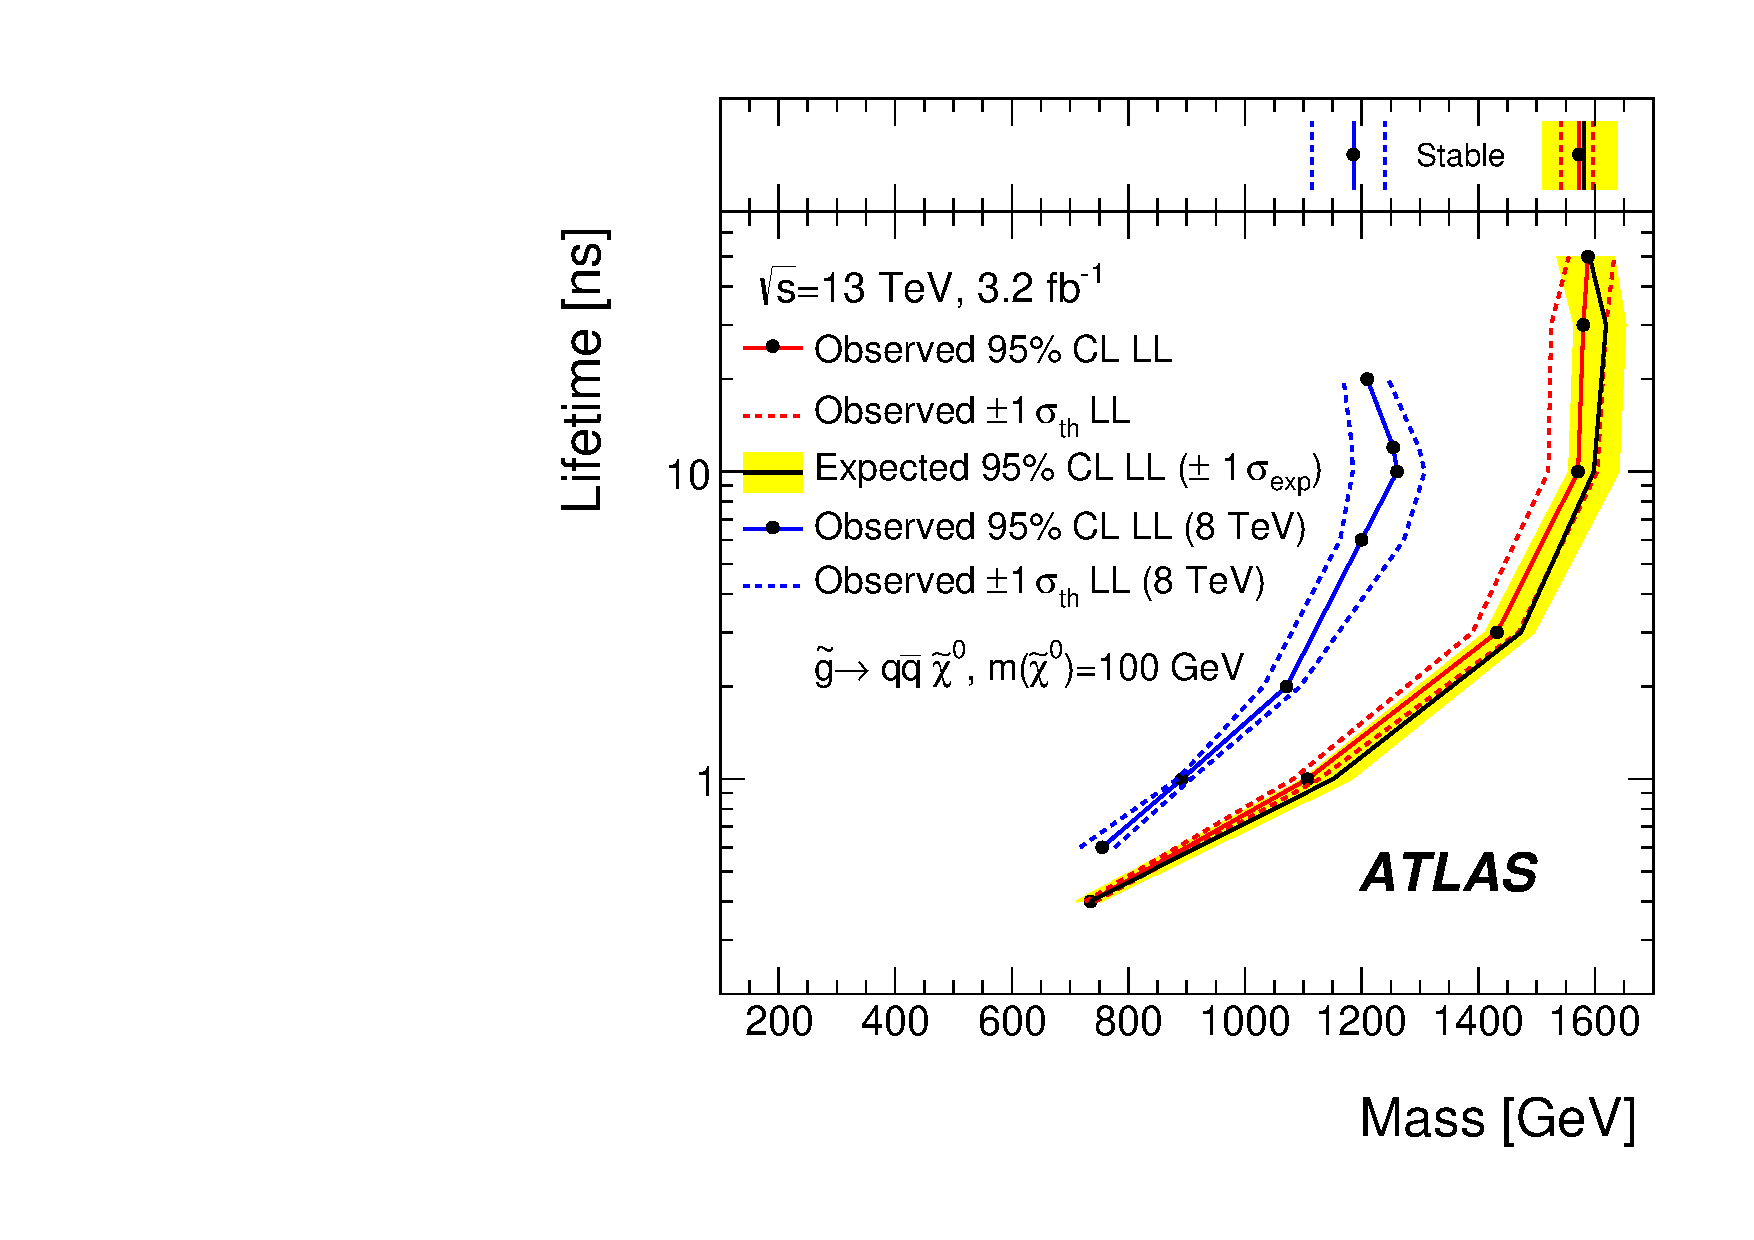
\includegraphics[width=\fullfig]{figures/taumass_exclusion.pdf}  
\caption{The excluded range of masses as a function of gluino lifetime. The expected lower limit (LL), with its experimental $\pm 1 \sigma$ band, is given with respect to the nominal theoretical cross-section. The observed 95\% LL obtained at $\sqrt{s} = 8$~\TeV~\cite{SUSY-2014-09} is also shown for comparison.}
\label{fig:mass_limits}
\end{figure}

% ----------------------------------------

\section{Context for Long-Lived Searches}
This search plays an important role in the current, combined \ac{ATLAS} search for long lived particles.
The mass limits provided by various \ac{ATLAS} searches for long-lived gluino \rhadrons can be seen in Figure~\ref{fig:combined_rhadrons}.
This search provides the most competitive limit for lifetimes between 3 ns up through very long lifetimes, where it is still competitive with dedicated searches for stable particles.
The limits placed on gluino production are very similar to the limits on promptly decaying models.

\begin{figure}[htbp]
\centering
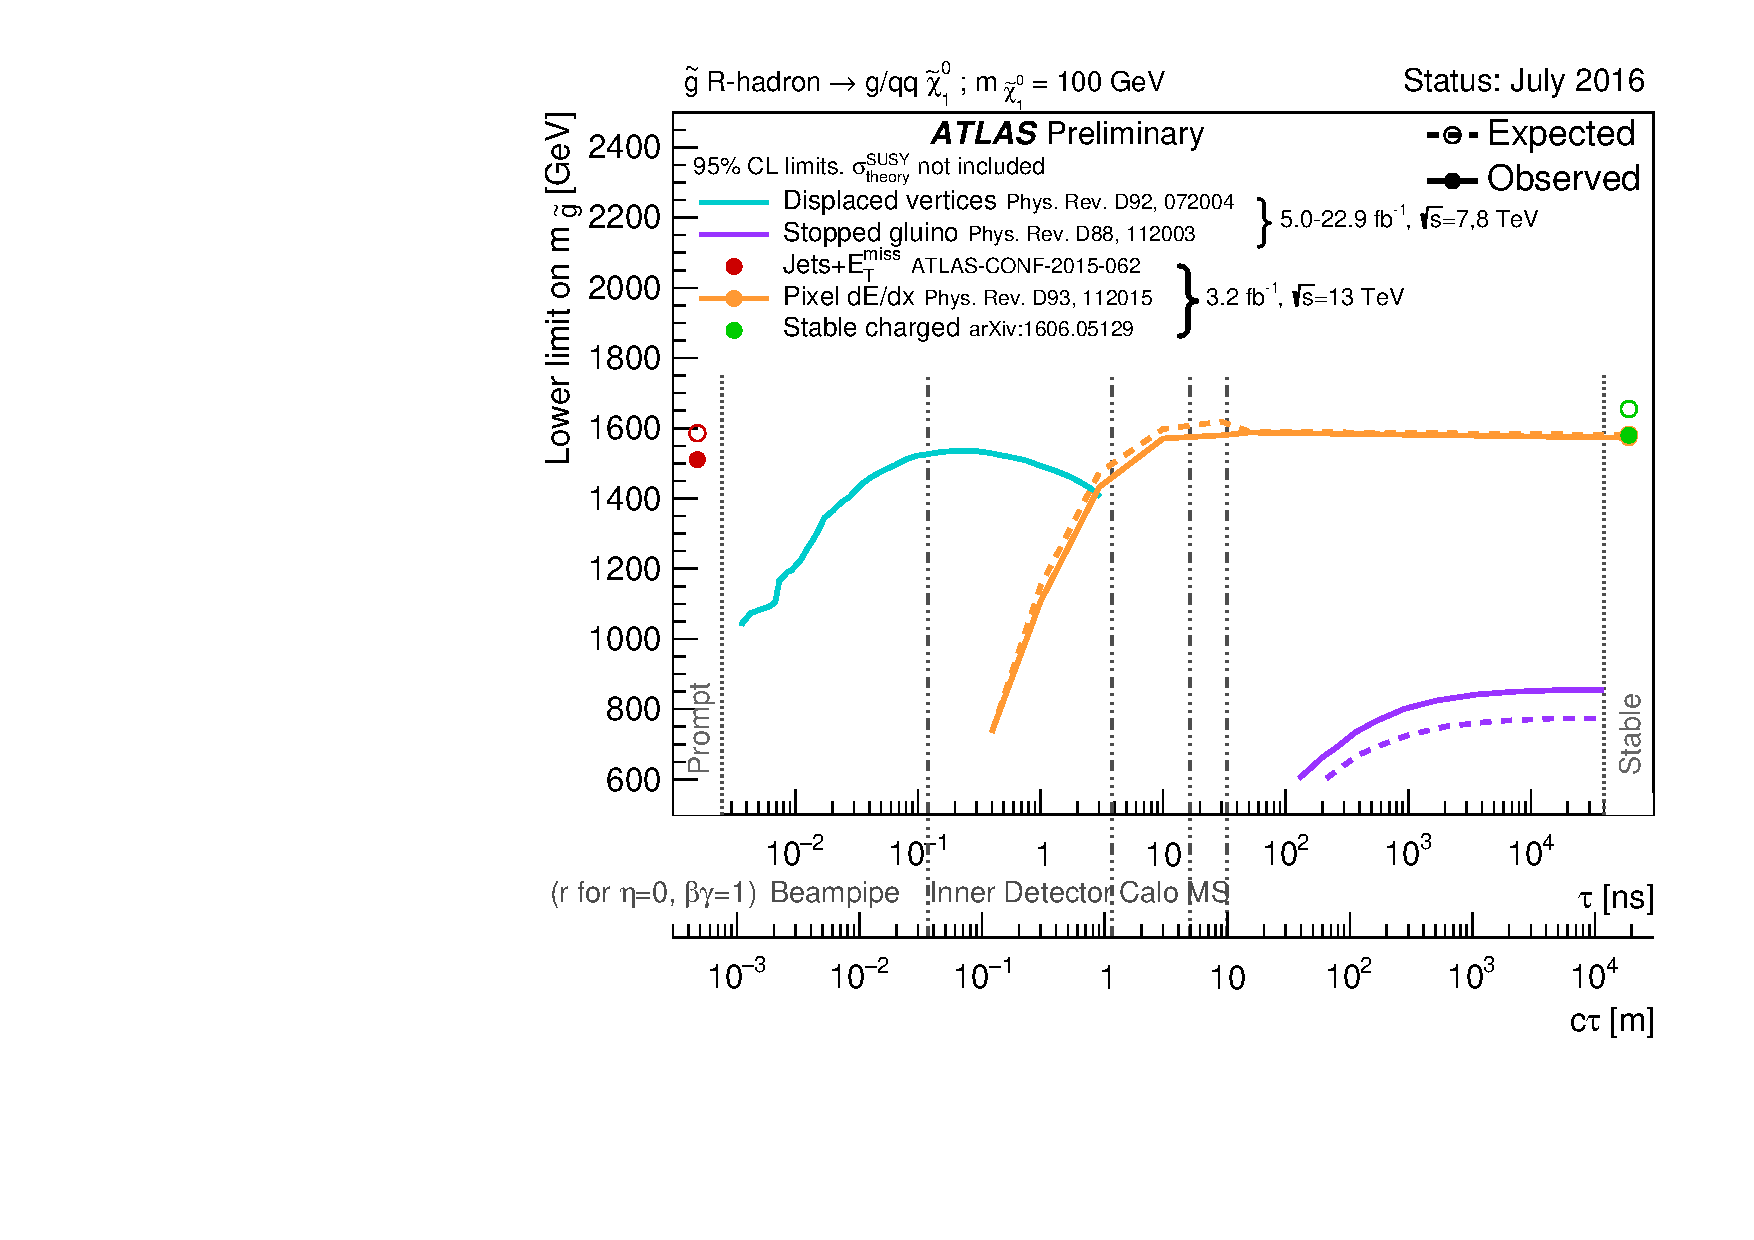
\includegraphics[width=\fullfig]{figures/combined_rhadrons.pdf}  
\caption{The constraints on the gluino mass as a function of lifetime for a split-supersymmetry model with the gluino \rhadrons decaying into a gluon or light quarks and a neutralino with mass of 100 GeV. The solid lines indicate the observed limits, while the dashed lines indicate the expected limits. The area below the curves is excluded. The dots represent results for which the particle is assumed to be prompt or stable.}
\label{fig:combined_rhadrons}
\end{figure}


% ----------------------------------------
